% Licencia y derechos: consulte ../../LICENSE-CC-BY-4.0.
% Las figuras y demás materiales de terceros pueden tener derechos separados y deben identificarse.

\chapter{Retroalimentación} %p129
\section{Introducción} %p129

Una de las desventajas mayores de los componentes electrónicos es su sensibilidad a la temperatura y la dificultad de fabricar unidades que se reproduzcan exactamente igual, lo cual hace variable las características de los mismos.

Por medio de la retroalimentación vamos a crear sistemas cuyas características globales sean inmunes a la variabilidad de los valores de los elementos electrónicos. En particular, vamos a conseguir amplificadores cuya ganancia dependa solo de la relación de dos resistencias y podamos resistencias de entrada y salida tan pequeñas que las aproximemos a cero, o resistencias de entrada tan grandes que las aproximemos a infinito.

La retroalimentación tiene además los siguientes efectos:

\begin{itemize}
	\item Aumenta enormemente el ancho de banda del amplificador, bajando la frecuencia de corte baja y aumentando la frecuencia de corte alta en la misma proporción que disminuye la ganancia, conservándose así el producto ganancia-ancho de banda.
	\item Permite reducir enormemente ruido y distorsión producida interna en el amplificador.
\end{itemize}

\section{El lazo de retroalimnentación} %p129

En la Figura \ref{fig:retro_estructura-general} se muestra la estructura básica de retroalimentación.

\begin{figure}[h]
	\centering
	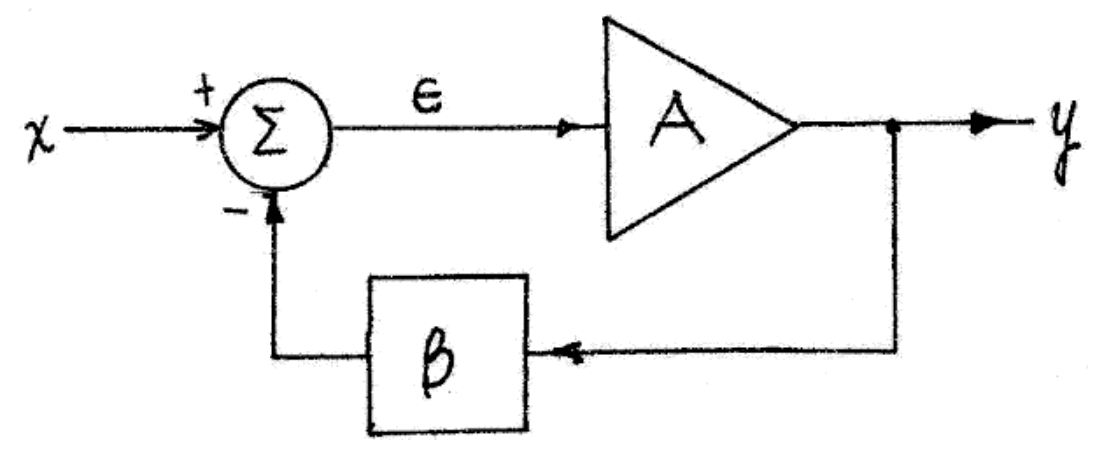
\includegraphics[width=0.9\linewidth]{_fig/retro_estructura-general.png}
	\caption{Estructura General de Retroalimentación}
	\label{fig:retro_estructura-general}
\end{figure}

Llamemos \( X \) a la señal de entrada, \( Y \) a la señal de salida, entonces se toma una muestra de la señal de salida, para retroalimentar una fracción, \( \beta Y \), a la entrada donde se compara con la señal de entrada genera así una diferencia \( e \). Esta diferencia es amplificada por \( A \) para generar la salida.

Entonces:

\[
e = x - \beta y
\]

\[
y = A e = A ( x - \beta y )
\]

\[
y + A \beta y = A x
\]

\[
y ( 1 + A \beta ) = A x
\]

\begin{equation}
	\frac{y}{x} = \frac{A}{1 + A \beta}
	\label{eq:retro1}
\end{equation}		

La ecuación \ref{eq:retro1} es la relación clásica de la retroalimentación. \( A \) generalmente representa un circuito activo con una relación muy elevada entre la salida y la entrada. \( \beta \) generalmente es un circuito pasivo. El producto \( A \beta \) tiene que ser adimensional. 

Si \( A \) y \( \beta \) son del mismo signo, el producto es positivo y corresponde a retroalimentación negativa. En cambio, si \( A \) y \( \beta \) son de signo contrario, se tiene retroalimentación positiva, lo que puede llevar a un sistema inestable.

Generalmente, \( A \beta \gg 1 \), de modo que:

\begin{equation}
	\frac{1}{1 + A \beta} \approx \frac{1}{A \beta}
	\label{eq:retro2}
\end{equation}

de aquí se destaca el mayor atributo de la retroalimentación en el sentido de que, en estas condiciones, la ganancia en el lazo cerrado, \( \frac{A}{1 + A \beta} \), es aproximadamente independiente de la ganancia en lazo abierto, \( A \), y depende únicamente de \( \beta \), que normalmente es un circuito pasivo, cuyas características son relarivamente invariables.

El efecto beneficioso sobre la distorsión o el ruido puede demostrarse por medio del diagrama de bloques, como el de la Figura \ref{fig:retro_estructura-general-ruido}, donde se ha introducido una señal de ruido \( n \).

\begin{figure}[h]
	\centering
	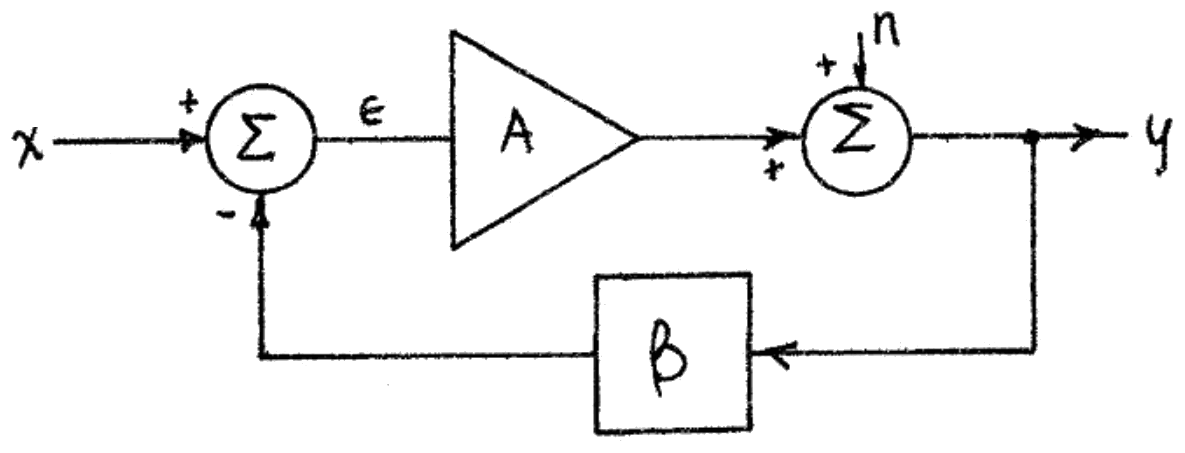
\includegraphics[width=0.9\linewidth]{_fig/retro_estructura-general-ruido.png}
	\caption{Sistema de Retroalimentación con Ruido}
	\label{fig:retro_estructura-general-ruido}
\end{figure}

Para hallar \( y \) en este caso aplicamos superposición, de donde:

\[
x_x = Ax(1 + A \beta)
\]

Para \( y_n \), se tiene:

\[
e = - \beta y_n
\]

\[
y_n = n + (-A \beta) y_n
\]

\[
y_n (1 + A \beta) = n
\]

\begin{equation}
	y_n = \frac{n}{1 + A \beta}
\end{equation}

es decir, a pesar el ruido se ha introducido en la misma puerta de salida, pero su componente en \( y_n \) se ve reducido por el factor \( 1 / (1 + A \beta) \).

\section{Análisis de los sistemas retroalimentados con métodos clásicos} %p131

A continuación, vamos a ver circuitos conocidos para demostrar cómo la retroalimentación puede tener los siguientes efectos:

\begin{itemize}
	\item - Aumenta el ancho de banda.
	\item Reduce la resistencia de entrada en algunos casos y la aumenta en otros.
	\item Reduce la resistencia de salida en algunos casos y la aumenta en otros.
\end{itemize}

Muchos de los circuitos que hemos visto han sido circuitos con retroalimentación, como por ejemplo, las configuraciones con Amplificador Operacional de la Figura \ref{fig:retro_gain}. La resistencia \( R_2 \) establece una comunicación de la salida con la entrada.

\begin{figure}[h]
	\centering
	\subfloat[Ganancia Negativa]
	{
		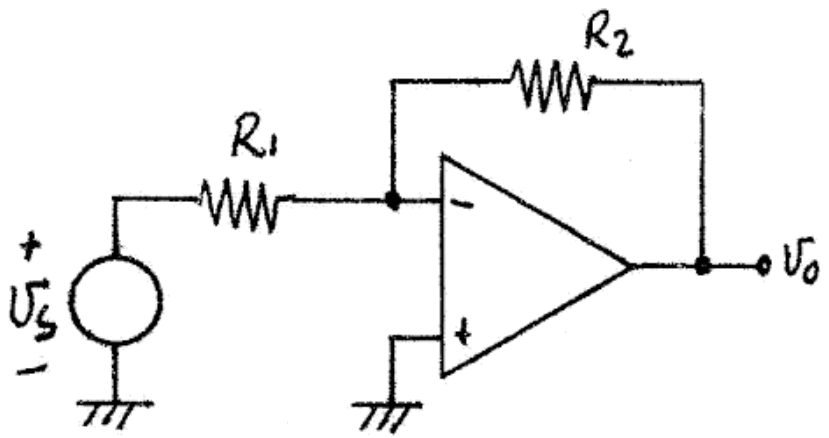
\includegraphics[width=0.4\linewidth]{_fig/retro_gain-neg.png}
		\label{fig:retro_gain-neg}
	}
	\subfloat[Ganancia Positiva]
	{
		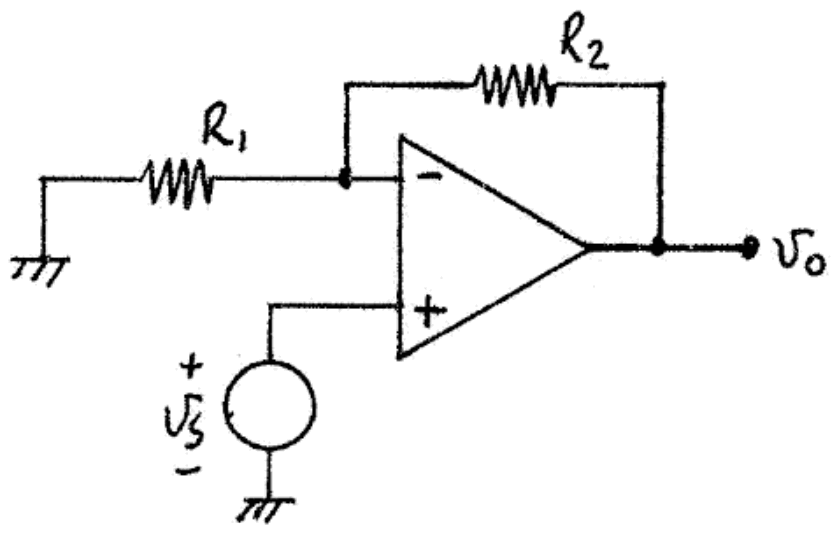
\includegraphics[width=0.4\linewidth]{_fig/retro_gain-pos.png}
		\label{fig:retro_gain-pos}
	}
	\caption{Amplificadores con Amplificador Operacional}
	\label{fig:retro_gain}
\end{figure}

\begin{figure}[h]
	\centering
	\subfloat[Modelo]
	{
		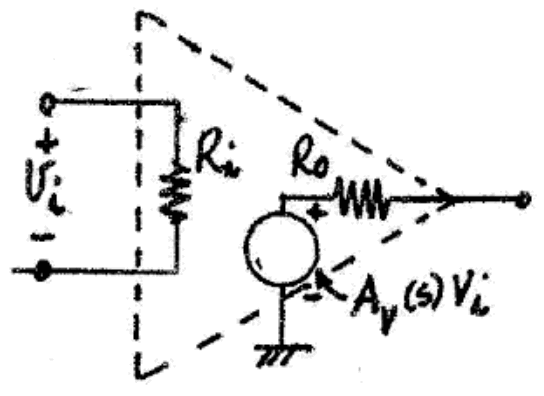
\includegraphics[width=0.4\linewidth]{_fig/retro_741-model.png}
		\label{fig:retro_741-model}
	}
	\subfloat[Respuesta de frecuencia]
	{
		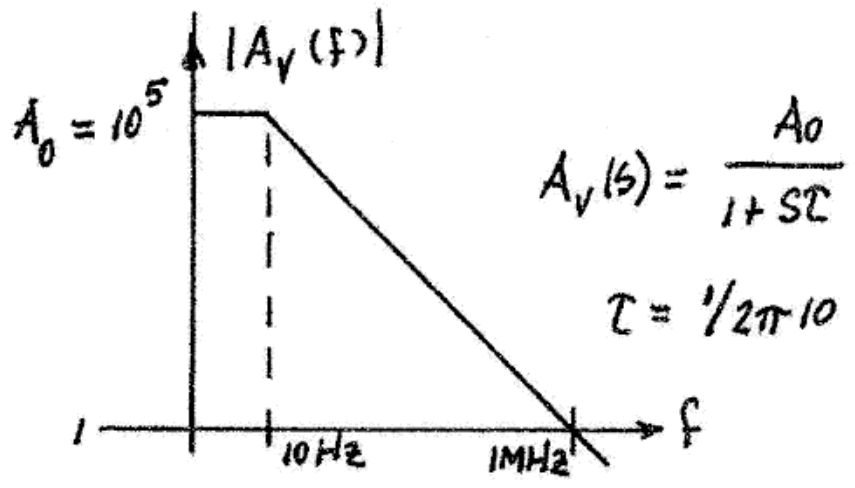
\includegraphics[width=0.4\linewidth]{_fig/retro_741-resp.png}
		\label{fig:retro_741-resp}
	}
	\caption{Modelo de un Amplificador Operacional con su Respuesta de Frecuencia}
	\label{fig:retro_741}
\end{figure}

Analicemos de nuevo estos circuitos. En la Figura \ref{fig:retro_741} se muestra el modelo a utilizar del amplificador operacional. Como valores para los elementos utilizamos las características del \textbf{uA741}, es decir:

\begin{itemize}
	\item Ganancia en lazo abierto de \( 100k \) (\( A_{vo} \)).
	\item Ancho de banda de \( 10 \) Hz (\( f_H = \frac{1}{2\pi \tau} \)).
	\item Resistencia de entrada de \( 6 M \Omega (R_i) \).
	\item Resistencia de salida de \( 25 M \Omega (R_o) \).
\end{itemize}

Veamos primero el efecto del ancho de banda con el circuito de la Figura \ref{fig:retro_741-model}. Para el modelo del operacional, consideramos su respuesta de frecuencia limitada, pero despreciamos por ahora el efecto que puede tener la resistencia de entrada y la resistencia de salida nos deja con el circuito equivalente de la Figura \ref{fig:retro_opamp-equiv}.

\begin{figure}[h]
	\centering
	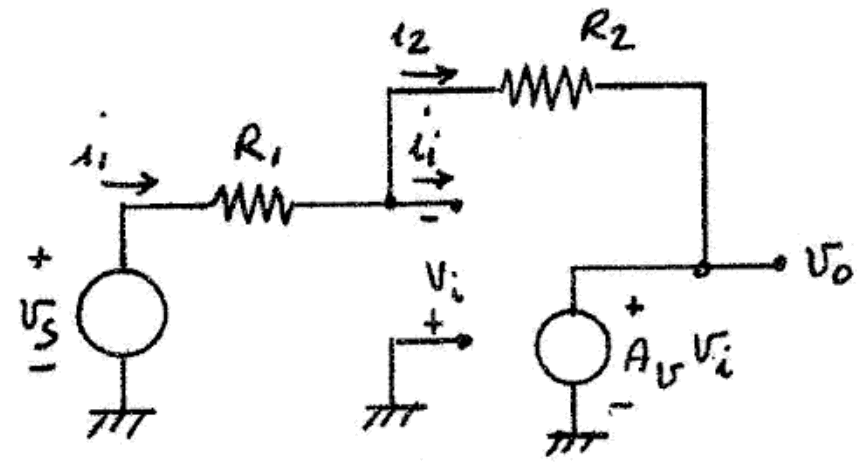
\includegraphics[width=0.9\linewidth]{_fig/retro_opamp-equiv.png}
	\caption{OpAmp Circuito Equivalente}
	\label{fig:retro_opamp-equiv}
\end{figure}

A la entrada se tiene:

\[
-v_i = \frac{-v_o}{A_v}
\]

Entonces,

\[
i_1 = \frac{v_s - (-v_o / A_v)}{R_1}
\]

\[
= \frac{v_s + v_o / A_v}{R_1}
\]

Aún consideramos \( R_i = \infty \) y \( R_o = 0 \). Entonces,

\[
i'_i = 0, \quad i_2 = i_1, \quad y \quad v_o = A_v v_i
\]

De modo que,

\[
v_o = -v_i - i_2 R_2
\]

\[
= -v_i - \left( \frac{v_s + v_o / A_v}{R_1} \right) R_2
\]

\[
= \frac{-v_o}{A_v} - \frac{v_s R_2}{R_1} - (\frac{v_o}{A_v})(\frac{R_2}{R_1})
\]

De donde:

\begin{equation}
	\frac{v_o}{v_s} = \frac{-R_2 / R_1}{1 + (1 + R_2 / R_1) / A_v}
\end{equation}

Ahora reemplazamos \( A_v = A_{v0} (1 + j f / f_{a0}) \), nos queda:

\[
\frac{v_o}{v_s} = -\left(\frac{R_2}{R_1}\right) \left( \frac{1}{1 + (1 + R_2/R_1)(1 + j f / f_{a0}) / A_{v0}} \right)
\]

\[
= -\left(\frac{R_2}{R_1}\right) \frac{1}{1 + (1 + R_2/R_1)/A_{v0} + (1 + R_2/R_1) j f / f_{a0} A_{v0}}
\]

Si \( A_{v0} \gg 1 + R_2 / R_1 \), y despreciamos ese término, entonces nos queda:

\[
\frac{v_o}{v_s} \approx -\left(\frac{R_2}{R_1}\right) \frac{1}{1 + j f (1 + R_2/R_1) / A_{v0} f_{a0}}
\]

De donde se desprende que la frecuencia de corte de la configuración, \( f_{corte} \), el coeficiente de \( j f \), viene dado por:

\[
f_{corte} = \frac{A_{v0} f_{a0}}{(1 + R_2 / R_1)} = \frac{f_T}{(1 + R_2 / R_1)}
\]

De forma semejante, uno podría analizar la configuración del amplificador con ganancia positiva, y el análisis daría que la ganancia de DC es igual a \( 1 + R_2/R_1 \), y que la frecuencia de corte es igual a la expresión anterior.

\subsection{Ejemplo}

Considere un A.O. con \( f_{a0} = 1 \) MHz. Hallar la frecuencia de corte del amplificador en lazo cerrado con ganancias de \( +1000, +100, +10, +1, -1, -10, -100, -1000 \).

\subsubsection{Solución}

\begin{table}[h]
	\centering
	\begin{tabular}{|c|c|c|c|}
		\hline
		\textbf{Ganancia en lazo cerrado} & \( R_2 / R_1 \) & \( f_{corte} \) & \textbf{Prod. \( A_v \) x BW} \\
		\hline
		1000  & 999  & 1 kHz   & 1 MHz  \\
		100   & 99   & 10 kHz  & 1 MHz  \\
		10    & 9    & 100 kHz & 1 MHz  \\
		1     & 0    & 1 MHz   & 1 MHz  \\
		-1    & 1    & 0.5 MHz & 0.5 MHz \\
		-10   & 10   & 90.9 kHz & 0.9 MHz \\
		-100  & 100  & 9.9 kHz & 0.99 MHz \\
		-1000 & 1000 & 1 kHz   & 1 MHz  \\
		\hline
	\end{tabular}
	\caption{Frecuencia de corte y producto ganancia-ancho de banda para diferentes configuraciones}
\end{table}

En resumen, la ganancia disminuye y la frecuencia de corte alta aumenta con retroalimentación. Sobre la misma respuesta de frecuencia en lazo abierto del amplificador operacional (amplificador en lazo abierto), puede trazarse la respuesta del amplificador con retroalimentación, en la Figura \ref{fig:retro_741-resp-misc}, muestra que la frecuencia de corte con retroalimentación se encuentra como la intersección de la ganancia con retroalimentación con la característica sin retroalimentación.

\begin{figure}[h]
	\centering
	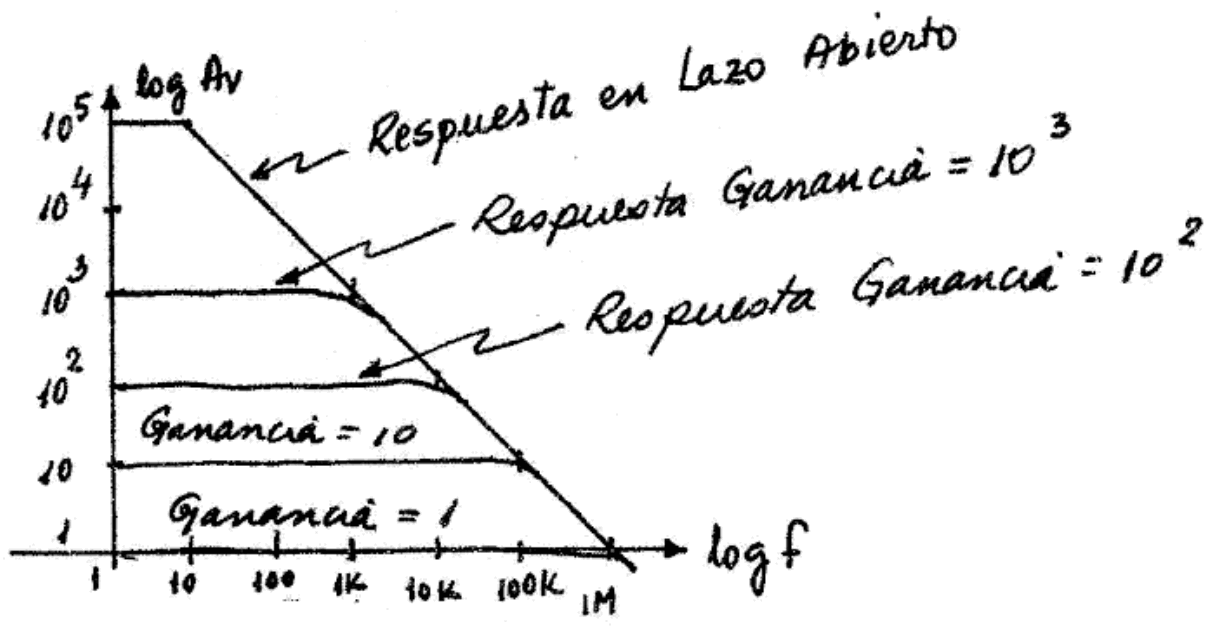
\includegraphics[width=0.9\linewidth]{_fig/retro_741-resp-misc.png}
	\caption{Respuesta en lazo abierto y con retroalimentación}
	\label{fig:retro_741-resp-misc}
\end{figure}

Consideramos ahora el efecto sobre la resistencia de entrada del mismo amplificador, tomando su \( R_i' \) en cuenta. Se muestra un circuito equivalente en la Figura \ref{fig:retro_741-with-retro}.

\begin{figure}[h]
	\centering
	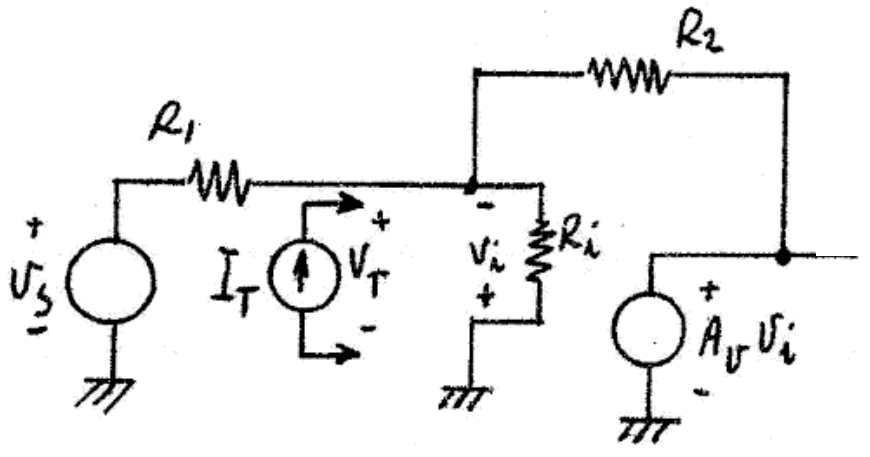
\includegraphics[width=0.9\linewidth]{_fig/retro_741-with-retro.png}
	\caption{Circuito equivalente con retroalimentación}
	\label{fig:retro_741-with-retro}
\end{figure}

Del circuito se obtiene:

\[
I_T + v_i / R_i' + (A_v v_i - (-v_i)) / R_2 = 0
\]

\[
I_T = - v_i \left( \frac{1}{R_i'} + \frac{(A_v + 1)}{R_2} \right)
\]

Pero \( -v_i = v_T \), entonces:

\[
\frac{v_T}{I_f} = \frac{1}{\left( \frac{1}{R_i'} + \frac{(A_v + 1)}{R_2} \right)}
\]

\[
= \frac{R_i'}{\left( \frac{R_2}{(A_v + 1)} \right)}
\]

Se ha reducido la gran \( R_i \) sin retroalimentación (\(6 M\Omega\) para el 741), a una \( R \) de entrada muy pequeña \( \approx 0.1 \Omega \) si \( R_2 = 10k\Omega \) y \(A_0 = 10^5 \); se ha aumentado la conductancia de entrada.

En cambio, para la configuración de ganancia positiva, que se muestra en la Figura \ref{fig:retro_conf-gain-pos}:

\[
v_i = I_T R_i
\]

\[
I_T = \frac{(E_T - v_i)}{R_1} + \frac{(E_T - v_i - A_v v_i)}{R_2}
\]

\begin{figure}[h]
	\centering
	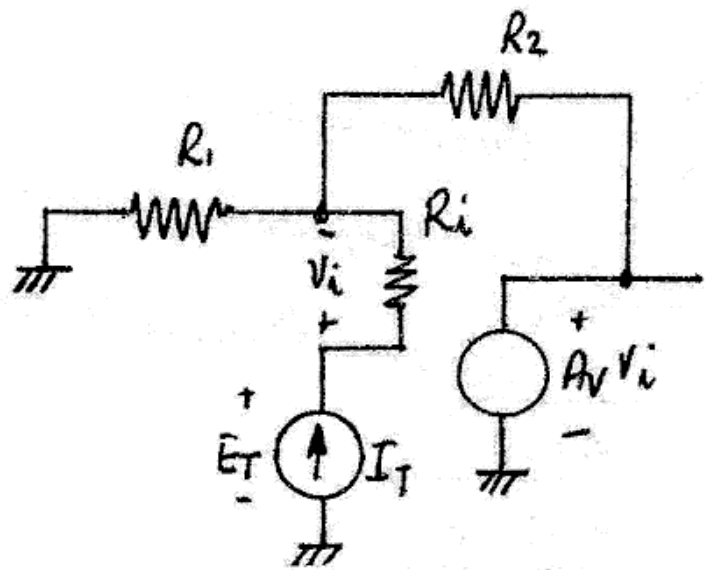
\includegraphics[width=0.7\linewidth]{_fig/retro_conf-gain-pos.png}
	\caption{Configuración de ganancia positiva}
	\label{fig:retro_conf-gain-pos}
\end{figure}

\[
I_T = E_T \left(\frac{1}{R_1} + \frac{1}{R_2} \right) - v_i \left(\frac{1}{R_1} + \frac{(1+A_v)}{R_2} \right)
\]

Luego,

\[
I_T \left(1 + R_i' \left(\frac{1}{R_1} + \frac{(1+A_v)}{R_2} \right) \right) = E_T \left(\frac{1}{R_1} + \frac{1}{R_2} \right)
\]

\[
R_{if} = \frac{E_T}{I_T} = R_1 \parallel R_2 \left(1 + R_i' \left(\frac{R_1}{R_2} + \frac{1+A_v}{R_2} \right) \right)
\]

Por ejemplo, si \( R_i = 6 M\Omega \), \( R_1 = 1 k\Omega \), \( R_2 = 10 k\Omega \), \( A_v = 10^5 \), nos da \( 54551 M\Omega \) (9091 veces mayor que \( R_i' \)).

Finalmente, determinemos \( R_{of} \) para el circuito de ganancia positiva o negativa. Nuevamente se considera \( A_v \) un valor limitado y por ahora consideramos \( R_f \) infinito. El circuito equivalente se muestra en la Figura \ref{fig:retro_calc-rof}.

\begin{figure}[h]
	\centering
	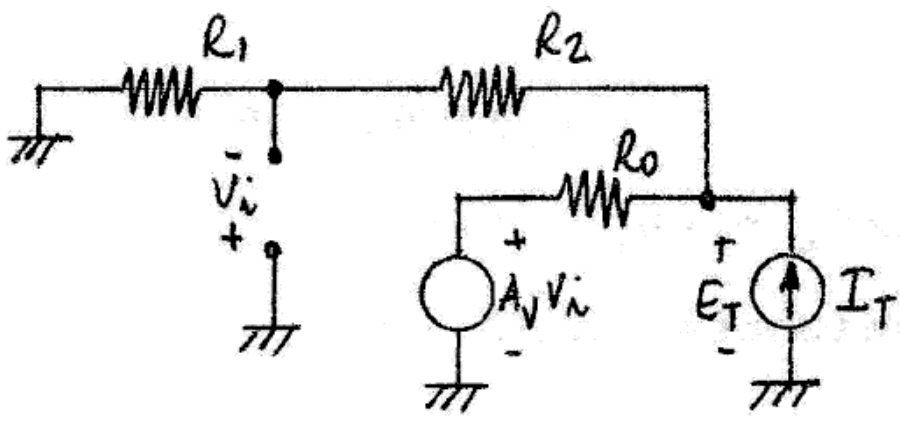
\includegraphics[width=0.9\linewidth]{_fig/retro_calc-rof.png}
	\caption{Circuito equivalente para determinar \( R_{of} \)}
	\label{fig:retro_calc-rof}
\end{figure}

Se tiene:

\[
I_T = \frac{(v_T - A_v v_i)}{R_0} + \frac{v_T}{(R_2 + R_1)}
\]

\[
- v_i = R_i V_T (R_1 + R_2)
\]

Entonces,

\[
I_T = V_T \left[ \left( \frac{1 + A_v R_i / (R_1 + R_2)}{R_0} \right) + \frac{1}{(R_1 + R_2)} \right]
\]

o

\[R_{of} = \frac{V_T}{I_T} = \frac{R_0}{(1 + A_v R_i / (R_1 + R_2))} \parallel (R_1 + R_2)
\]

\[
\approx \frac{R_0}{(1 + A_v R_i / (R_1 + R_2))}
\]

Ahora podemos utilizar valores finitos de \( R_0 \) y \( A_v \) para encontrar \( R_{of} \).

Si \( R_1 = 1k\Omega \), \( R_2 = 9k\Omega \), \( A_v = 100,000 \) y \( R_0 = 25\Omega \), da

\[
R_{of} \approx \frac{25}{(1 + 10^5 / 10)} \approx 25 \times 10^{-3} = 2.5 m\Omega
\]

Hemos demostrado los efectos de la retroalimentación sobre circuitos muy conocidos con herramientas también conocidas ("a pie").  
En las próximas secciones presentamos una metodología orientada especialmente a sistemas retroalimentados.  
Consiste en encontrar \( A \) y \( \beta \) por separado y utilizar el factor \( (1 + A\beta) \) para determinar la frecuencia de corte alta y baja, la resistencia de entrada y salida.  
De tal forma, se tendrá mayor intuición sobre por qué y cómo los sistemas retroalimentados consiguen su efecto, y de paso nos brindará una herramienta que frecuentemente será más eficaz para determinar las características del circuito.  

Por ahora hemos podido comprobar que la retroalimentación realmente tiene estos efectos.

\section{Cuatro configuraciones básicas con retroalimentación} %p137

La configuración básica con retroalimentación, la Figura 3.1, es una representación genérica de un sistema, de modo que los variables de entrada, salida y retroalimentación pueden ser cualquier parámetro, como por ejemplo, tensión, corriente, fase, frecuencia, etc. Por ahora, nuestro interés estará centrado en esos casos donde las variables son tensiones o corrientes. Para ellos:

\begin{enumerate}
	\item Si se muestrea la tensión de salida, Figura \ref{fig:retro_conf_muestreo-nodo}, entonces \( y = v \); esto se conoce como \textbf{muestreo de nodo} y tiene el efecto de reducir la resistencia del nodo de salida.
	\item En cambio, si se muestrea la corriente de salida, Figura \ref{fig:retro_conf_muestreo-lazo}, entonces \( y = i \); esto se conoce como \textbf{muestreo de lazo} y tiene el efecto de aumentar la resistencia del lazo de salida.
	\item Si se comparan tensiones a la entrada, Figura \ref{fig:retro_conf_comparacion-lazo}, entonces \( x = v \); esto se conoce como \textbf{comparación de lazo} y tiene el efecto de aumentar la resistencia del lazo de entrada.
	\item Finalmente, si se comparan corrientes a la entrada, Figura \ref{fig:retro_conf_comparacion-nodo}, entonces \( x = i \); esto se conoce como \textbf{comparación de nodo} y tiene el efecto de reducir la resistencia del nodo de entrada.
\end{enumerate}

\begin{figure}[h]
	\centering
	\subfloat[Muestreo de Nodo]
	{
		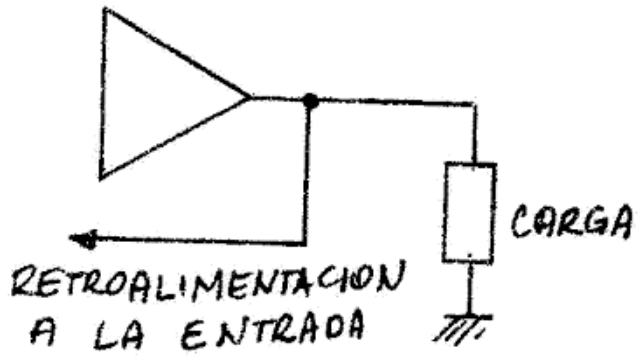
\includegraphics[width=0.22\linewidth]{_fig/retro_conf_muestreo-nodo.png}
		\label{fig:retro_conf_muestreo-nodo}
	}
	\subfloat[Muestreo de Lazo]
	{
		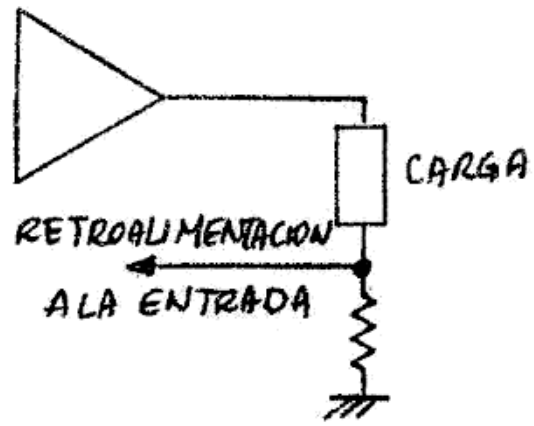
\includegraphics[width=0.22\linewidth]{_fig/retro_conf_muestreo-lazo.png}
		\label{fig:retro_conf_muestreo-lazo}
	}
	\subfloat[Comparación de Lazo]
	{
		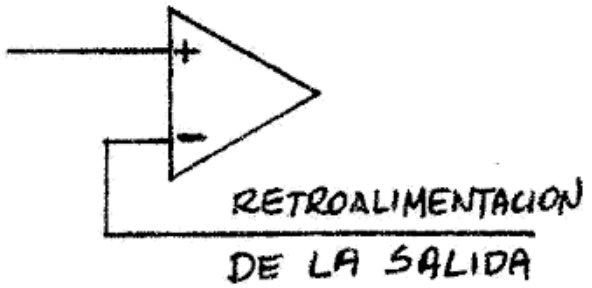
\includegraphics[width=0.22\linewidth]{_fig/retro_conf_comparacion-lazo.png}
		\label{fig:retro_conf_comparacion-lazo}
	}
	\subfloat[Comparación de Nodo]
	{
		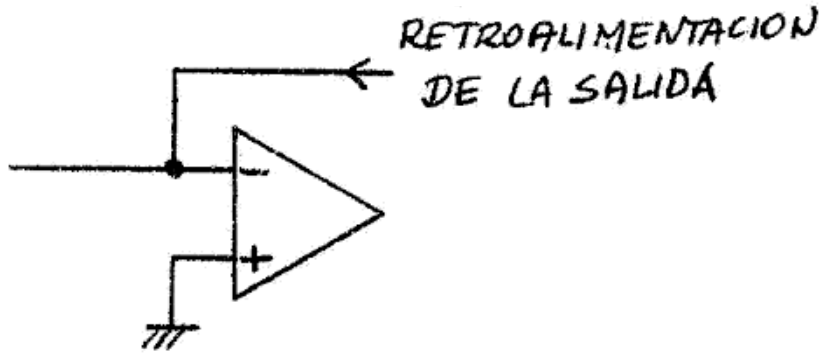
\includegraphics[width=0.22\linewidth]{_fig/retro_conf_comparacion-nodo.png}
		\label{fig:retro_conf_comparacion-nodo}
	}
	\caption{ Diagramas de tipos de muestreo y comparación}
	\label{fig:retro_conf}
\end{figure}

La combinación de uno de los dos tipos de muestreo a la combinación de uno de los dos tipos de comparación a la entrada da lugar a cuatro configuraciones de retroalimentación. En la Tabla 3.1 se hace un cuadro comparativo, donde se destaca el tipo de señal a la entrada y a la salida, el efecto sobre la resistencia de entrada y de salida, y el tipo de relación que resulta ser \(\beta\) y \(A\).

\begin{table}[h]
	\centering
	\begin{tabular}{|l|c|c|c|c|c|c|}
		\hline
		\textbf{Tipo de retroalimentación} & \textbf{S. \( y \)} & \textbf{S. \( x \)} & \( R_{of} \) & \( R_{if} \) & \( \beta \) & \( A \) \\
		\hline
		M. Nodo - Comp. de Lazo & \( v_o \) & \( v_s \) & dism. & aum. & \( v_f / v_o \) & \( v_o / v_s \) \\
		\hline
		M. Lazo - Comp. de Nodo & \( i_o \) & \( i_s \) & aum. & dism. & \( i_f / i_o \) & \( i_o / i_s \) \\
		\hline
		M. Nodo - Com[p.] de Nodo & \( v_o \) & \( i_s \) & dism. & dism. & \( i_f / v_o \) & \( v_o / i_s \) \\
		\hline
		M. Lazo - Comp. de Lazo & \( i_o \) & \( v_s \) & aum. & aum. & \( v_f / i_o \) & \( i_o / v_s \) \\
		\hline
	\end{tabular}
	\caption{Tabla 3.1. Cuadro Comparativo de los Tipos de Retroalimentación.}
	\label{tab:retro_comparativo}
\end{table}

A continuación, para cada tipo de retroalimentación vamos a mostrar tres figuras: en la primera, un esquema de interconexión de cuadripolos en su forma más general; en la segunda, un esquema de interconexión de cuadripolos más parecido a circuitos reales, donde se indican las conexiones a tierra; y finalmente, para cada tipo, un ejemplo de un circuito real, bien sea transistorizado o con amplificadores operacionales.

\subsection{Muestreo de Nodo - Comparación de Lazo} %p139

En la Figura \ref{fig:retro_m-nodo_c-lazo_a} se muestra el diagrama de bloques de este tipo de retroalimentación donde las señales de interés son las tensiones de salida y de entrada. La red \(\beta\) de retroalimentación devuelve una tensión \( v_f \) a la entrada que es una muestra de la tensión de salida \( v_o \); por lo tanto, \( \beta \) es una relación de tensiones.

En la Figura \ref{fig:retro_m-nodo_c-lazo_a} se muestra una comparación de lazo con muestreo de nodo.

\begin{figure}[h]
	\centering
	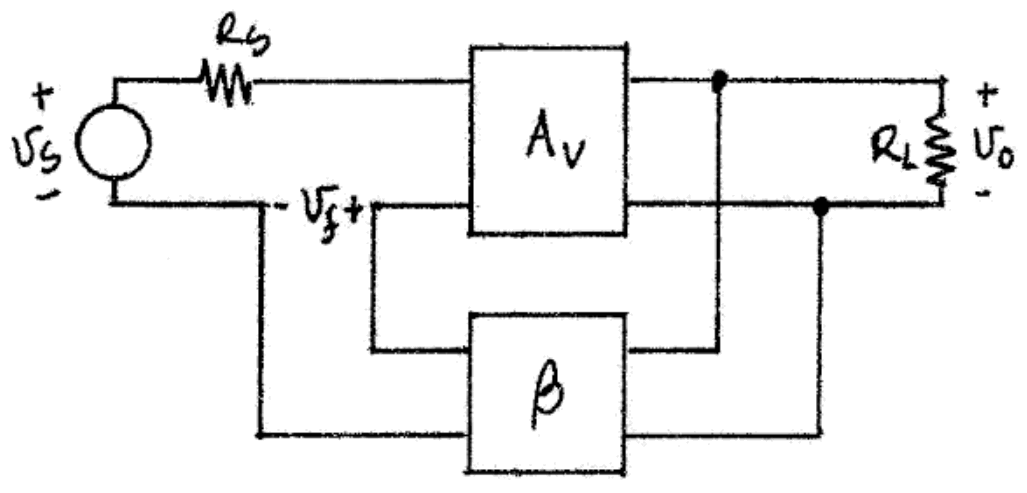
\includegraphics[width=0.6\linewidth]{_fig/retro_m-nodo_c-lazo_a.png}
	\caption{Muestreo de Nodo - Comparación de Lazo}
	\label{fig:retro_m-nodo_c-lazo_a}
\end{figure}

En la Figura \ref{fig:retro_m-nodo_c-lazo_b} se representa de nuevo este tipo de retroalimentación, pero ahora referenciando los cuadripolos a tierra. Además, se ha indicado dentro del bloque de \( \beta \) la configuración típica de esta como un divisor de tensión formado por dos resistencias.

\begin{figure}[h]
	\centering
	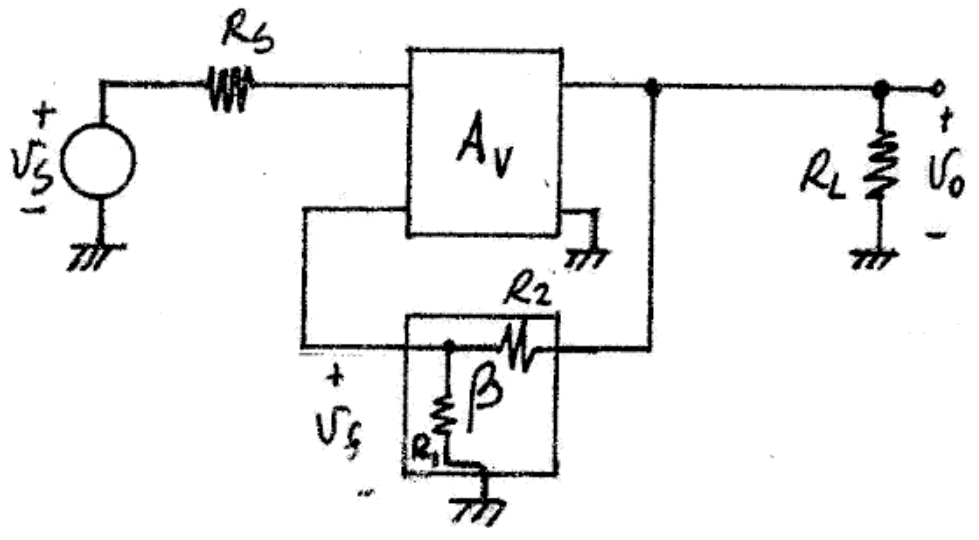
\includegraphics[width=0.6\linewidth]{_fig/retro_m-nodo_c-lazo_b.png}
	\caption{Muestreo de Nodo - Comparación de Lazo}
	\label{fig:retro_m-nodo_c-lazo_b}
\end{figure}

En la Figura \ref{fig:retro_m-nodo_c-lazo_c} se muestran dos ejemplos de circuitos con este tipo de retroalimentación.

\begin{figure}[h]
	\centering
	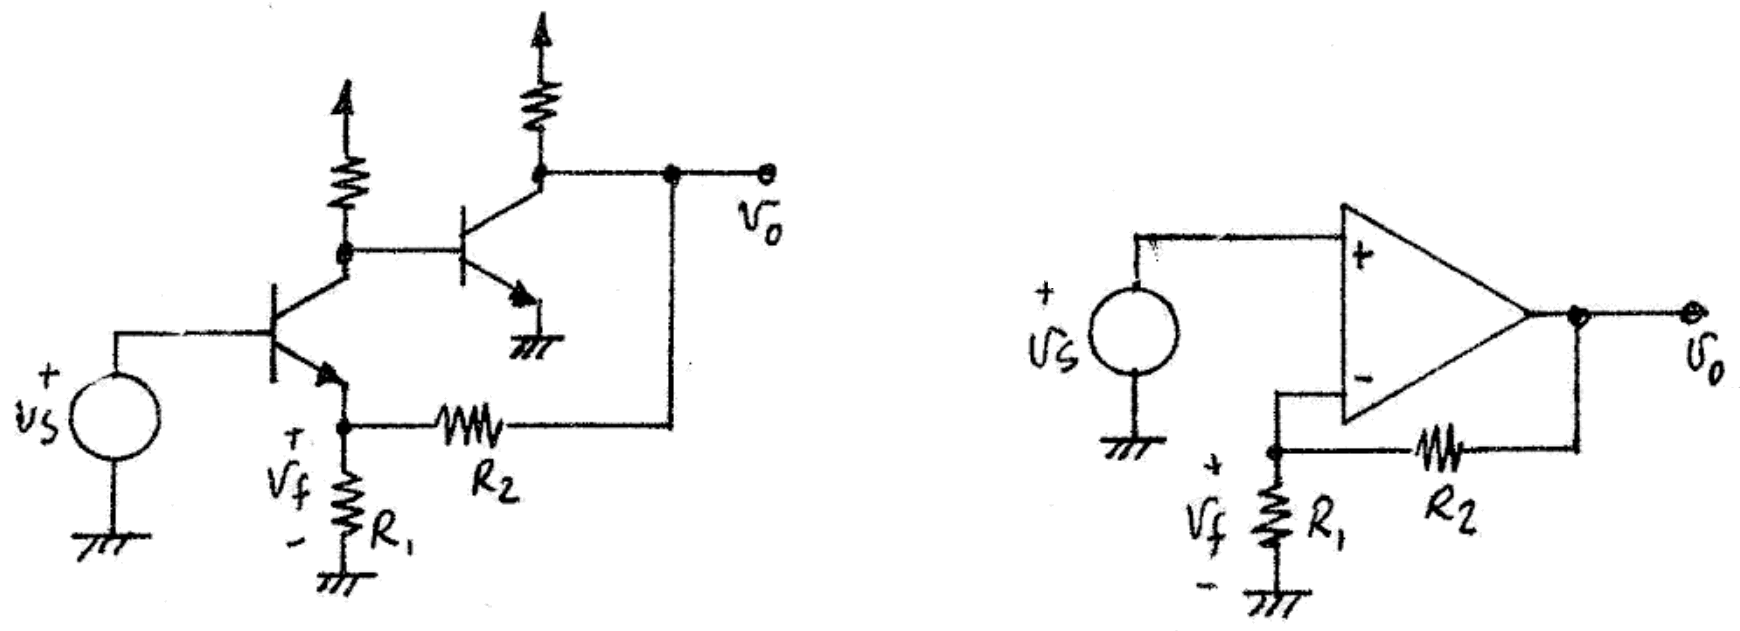
\includegraphics[width=0.8\linewidth]{_fig/retro_m-nodo_c-lazo_c.png}
	\caption{Muestreo de Nodo - Comparación de Lazo}
	\label{fig:retro_m-nodo_c-lazo_c}
\end{figure}

\subsection{Muestreo de Lazo - Comparación de Nodo} %p141

En la Figura \ref{fig:retro_m-lazo_c-nodo_a} se muestra el diagrama de bloques de este tipo de retroalimentación, donde las señales de interés son las corrientes de salida y de entrada. La red $\beta$ de retroalimentación devuelve una corriente $i_f$ a la entrada, que es una muestra de la corriente de salida $i_o$; Por lo tanto, $\beta$ es una relación de corrientes. A su vez, el bloque $A_I$ representa un amplificador de corrientes.

\begin{figure}[h]
	\centering
	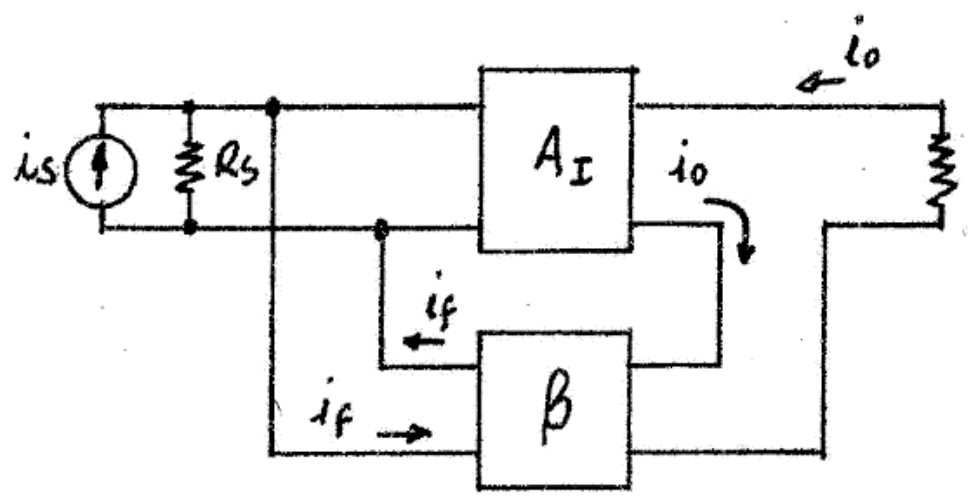
\includegraphics[width=0.6\linewidth]{_fig/retro_m-lazo_c-nodo_a.png}
	\caption{Muestreo de Lazo - Comparación de Nodo}
	\label{fig:retro_m-lazo_c-nodo_a}
\end{figure}

En la Figura \ref{fig:retro_m-lazo_c-nodo_b} se representa de nuevo este tipo de retroalimentación, pero ahora referenciando los cuadripolos a tierra. Además, se ha indicado dentro del bloque de $\beta$ la configuración típica de esta como un divisor de corriente formado por dos resistencias.

\begin{figure}[h]
	\centering
	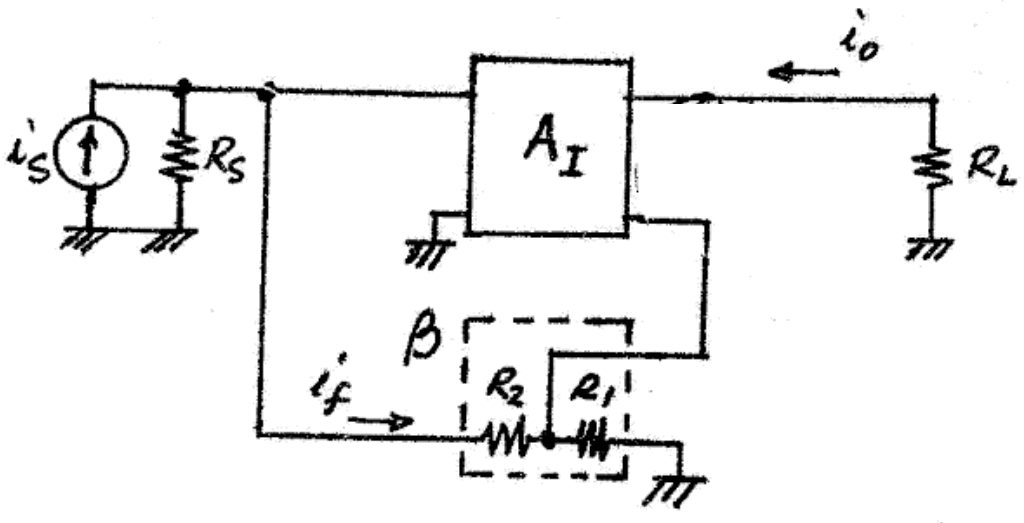
\includegraphics[width=0.6\linewidth]{_fig/retro_m-lazo_c-nodo_b.png}
	\caption{Muestreo de Lazo - Comparación de Nodo}
	\label{fig:retro_m-lazo_c-nodo_b}
\end{figure}

En la Figura \ref{fig:retro_m-lazo_c-nodo_c} se muestra un ejemplo de circuitos con este tipo de retroalimentación. En él se hace la distinción entre la corriente de salida, $i_0$, y la corriente que entra a la red $\beta$, $i_0'$.

\begin{figure}[h]
	\centering
	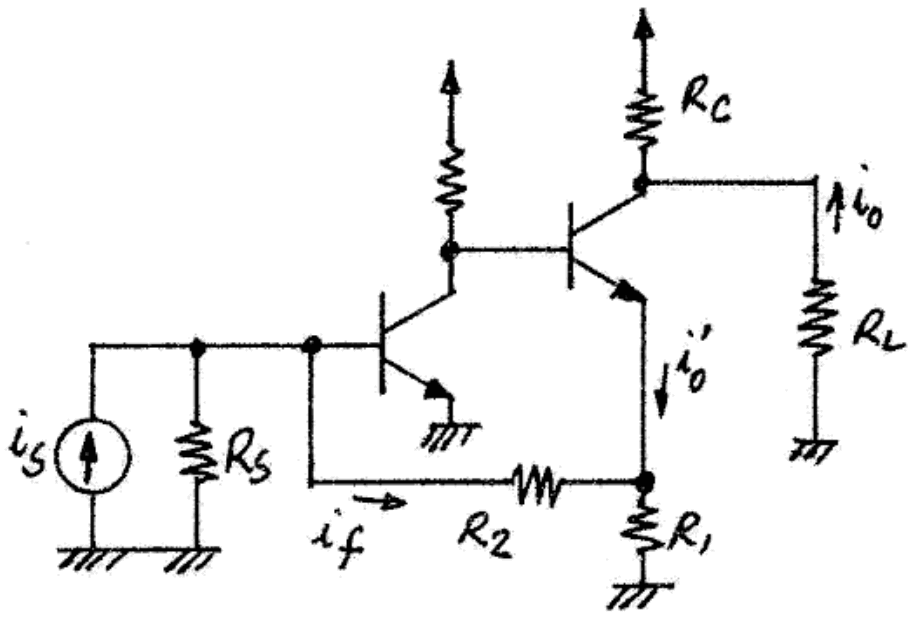
\includegraphics[width=0.6\linewidth]{_fig/retro_m-lazo_c-nodo_c.png}
	\caption{Muestreo de Lazo - Comparación de Nodo}
	\label{fig:retro_m-lazo_c-nodo_c}
\end{figure}

\subsection{Muestreo de Nodo - Comparación de Nodo} %p142

En la Figura \ref{fig:retro_m-nodo_c-nodo_a} se muestra el diagrama de bloques de este tipo de retroalimentación, donde las señales de interés son la tensión de salida y la corriente de entrada. La red $\beta$ de retroalimentación devuelve una corriente $i_f$ a la entrada, que es una muestra de la tensión de salida $v_0$. Por lo tanto, $\beta = i_f / v_0$, tiene unidades de conductancia. En cambio, el bloque $A$ representa una relación de tensión de salida en función de la corriente de entrada; $A_R = v_0 / i_s$, es decir, tiene unidades de resistencia.

\begin{figure}[h]
	\centering
	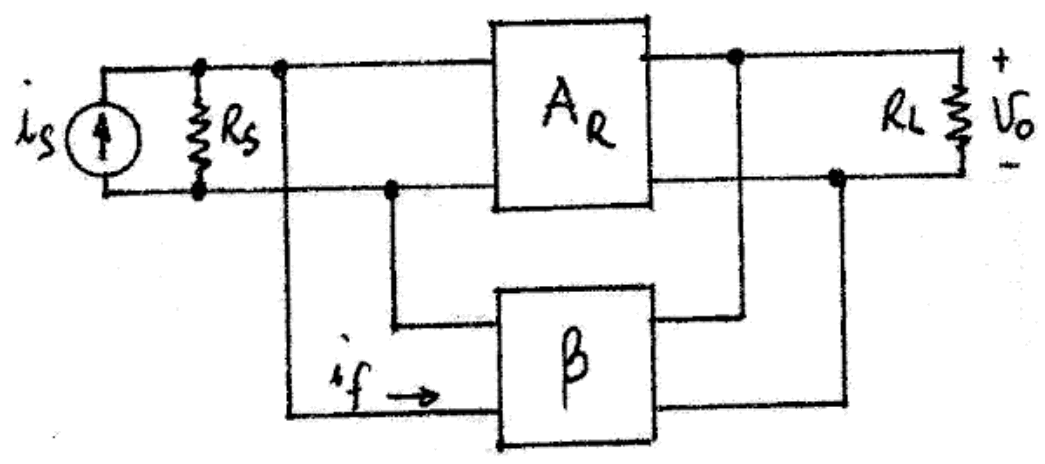
\includegraphics[width=0.6\linewidth]{_fig/retro_m-nodo_c-nodo_a.png}
	\caption{Muestreo de Nodo - Comparación de Nodo}
	\label{fig:retro_m-nodo_c-nodo_a}
\end{figure}

En la Figura \ref{fig:retro_m-nodo_c-nodo_b} se representa de nuevo este tipo de retroalimentación, pero ahora referenciando los cuadripolos a tierra. Además, ahora se ha indicado dentro del bloque de $\beta$ la configuración típica, que en este caso consiste simplemente de una resistencia.

\begin{figure}[h]
	\centering
	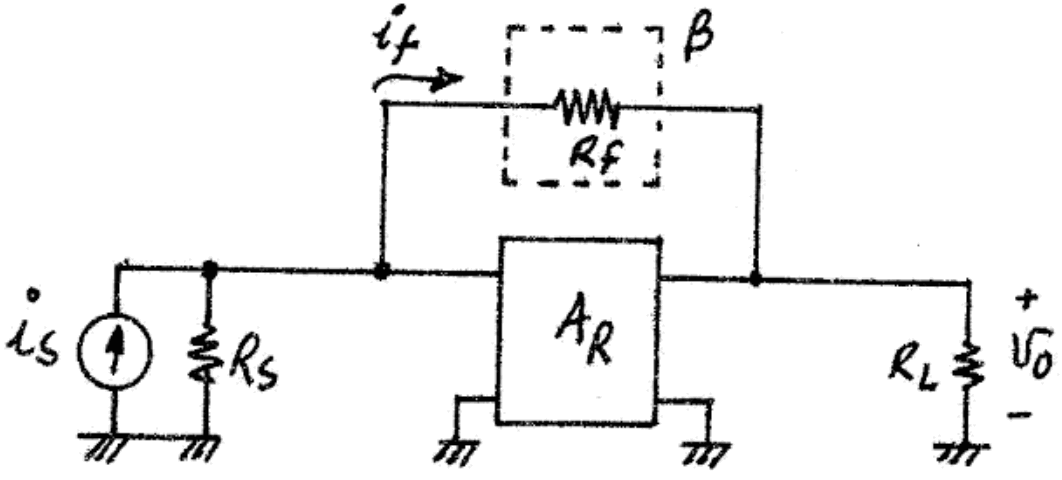
\includegraphics[width=0.6\linewidth]{_fig/retro_m-nodo_c-nodo.b.png}
	\caption{Muestreo de Nodo - Comparación de Nodo}
	\label{fig:retro_m-nodo_c-nodo_b}
\end{figure}

Además, en la Figura \ref{fig:retro_m-nodo_c-nodo_c} se muestran dos ejemplos de circuitos con este tipo de retroalimentación. Uno de ellos es la conocida configuración de ganancia negativa con el amplificador operacional.

\begin{figure}[h]
	\centering
	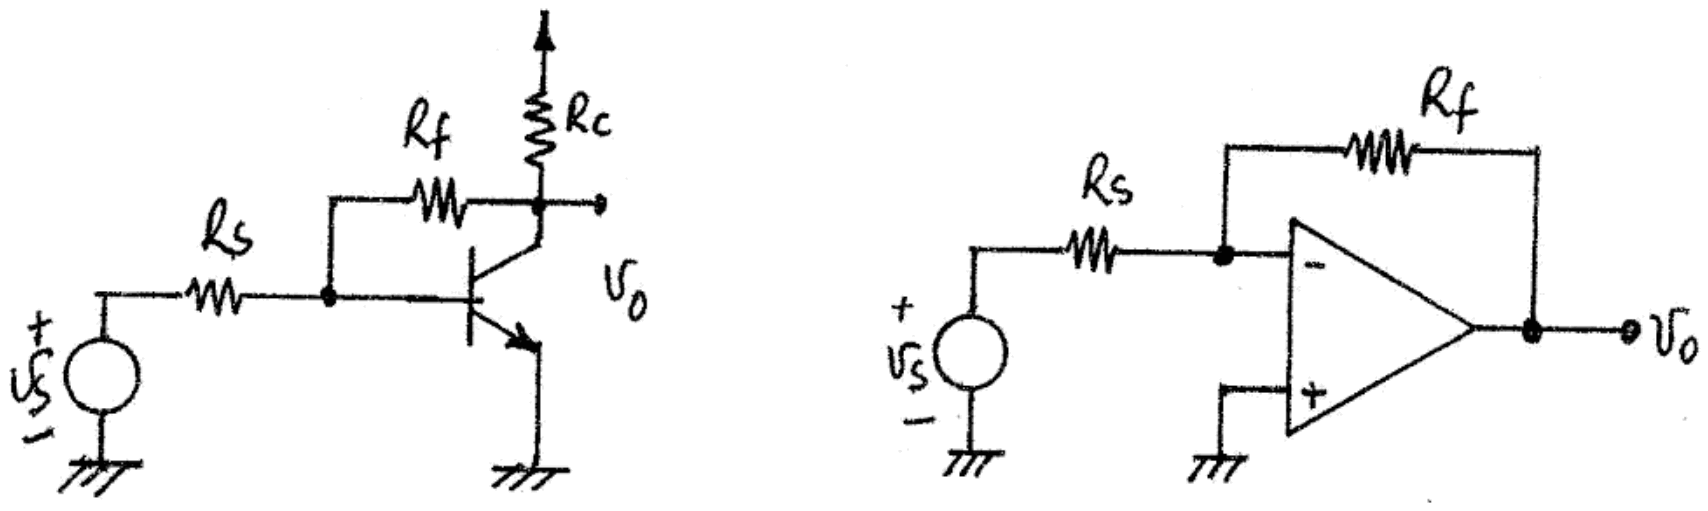
\includegraphics[width=0.6\linewidth]{_fig/retro_m-nodo_c-nodo_c.png}
	\caption{Muestreo de Nodo - Comparación de Nodo}
	\label{fig:retro_m-nodo_c-nodo_c}
\end{figure}

\subsection{Muestreo de Lazo - Comparación de Lazo} %p143

En la Figura \ref{fig:retro_m-lazo_c-lazo_a} se muestra el diagrama de bloques de este tipo de retroalimentación, donde las señales de interés son la corriente de salida y la tensión de entrada. La red $\beta$ de retroalimentación genera una tensión $v_f$ a la entrada, que es una muestra de la corriente de salida $i_o$; por lo tanto, $\beta = v_f / i_0$, tiene unidades de resistencia. En cambio, el bloque $A$ representa una relación de corriente de salida en función de la tensión de entrada, $A_G = i_o / v_s$, es decir, tiene unidades de conductancia.

\begin{figure}[h]
	\centering
	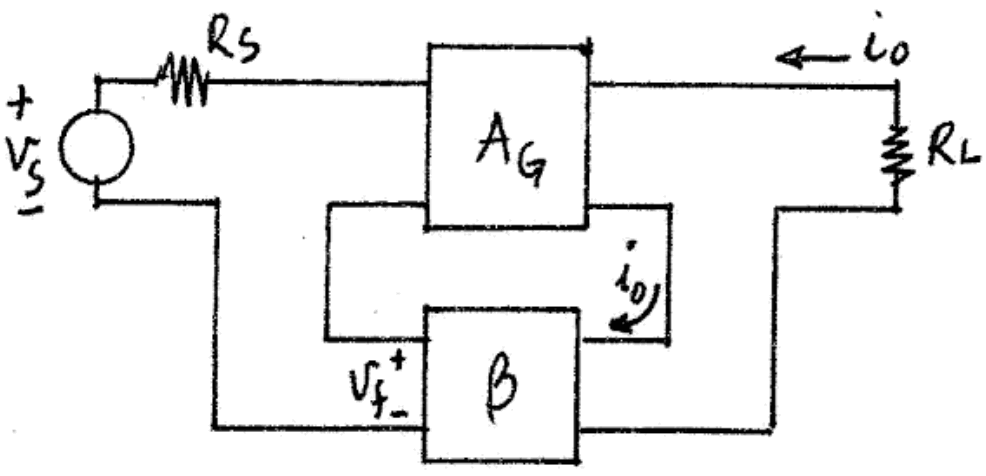
\includegraphics[width=0.8\linewidth]{_fig/retro_m-lazo_c-lazo_a.png}
	\caption{Muestreo de Lazo - Comparación de Lazo}
	\label{fig:retro_m-lazo_c-lazo_a}
\end{figure}

En la Figura \ref{fig:retro_m-lazo_c-lazo_b} se representa de nuevo este tipo de retroalimentación, pero ahora referenciando los cuadripolos a tierra. Además, ahora se ha indicado dentro del bloque de $\beta$ la configuración típica, que en este caso consiste simplemente en una resistencia.

\begin{figure}[h]
	\centering
	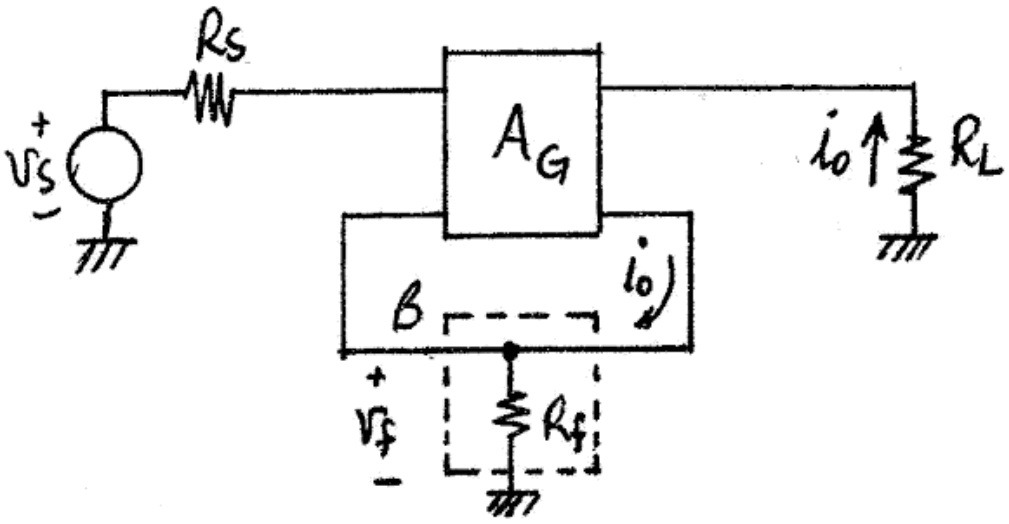
\includegraphics[width=0.8\linewidth]{_fig/retro_m-lazo_c-lazo_b.png}
	\caption{Muestreo de Lazo - Comparación de Lazo}
	\label{fig:retro_m-lazo_c-lazo_b}
\end{figure}

En la Figura \ref{fig:retro_m-lazo_c-lazo_c} se muestra un ejemplo de circuitos con este tipo de retroalimentación. Es la conocida configuración emisor común con $R_E$.

\begin{figure}[h]
	\centering
	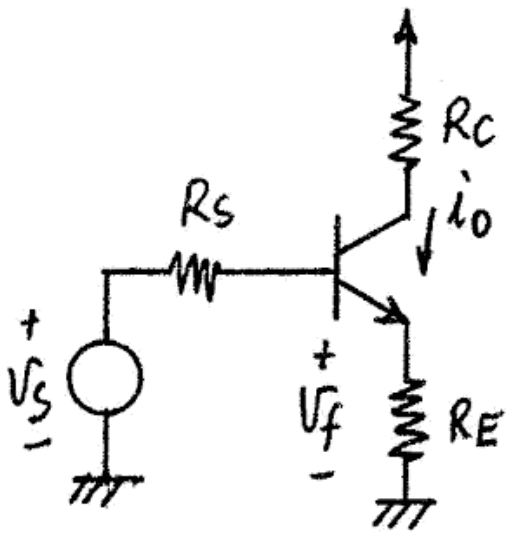
\includegraphics[width=0.6\linewidth]{_fig/retro_m-lazo_c-lazo_c.png}
	\caption{Muestreo de Lazo - Comparación de Lazo}
	\label{fig:retro_m-lazo_c-lazo_c}
\end{figure}

\section{Interpretación de Circuitos Como Lazo Cerrado con Retroalimentación} %p145

A continuación, presentaremos una metodología de análisis especial para circuitos con retroalimentación. Nos determinará condiciones necesarias que deben cumplirse, que permitirá hallar $A$ y $\beta$ por separado.

\subsection{Muestreo de Nodo - Comparación de Nodo} %p145

En la Figura \ref{fig:retro_m-nodo_c-nodo} se muestra un esquema idealizado de la retroalimentación Muestreo de Nodo - Comparación de Nodo. La resistencia de la fuente se ha incorporado a la $R_i$ del amplificador, y así mismo la $R_L$ de carga se ha incorporado con la $R_o$ de salida del amplificador (comparar con la Figura \ref{fig:retro_m-nodo_c-nodo_a}). En el diagrama tenemos el cuadrito perteneciente al amplificador sin retroalimentación $A$, con su resistencia de entrada sin retroalimentación, $R_i$, y su resistencia de salida sin retroalimentación, $R_o$. También se muestra un cuadrito de la retroalimentación $\beta$; tenemos la fuente de entrada $I_s$, la corriente retroalimentada $I_f$, la diferencia $I_i$, y el voltaje de salida $V_o$. Muy parecido al diagrama ideal.

\begin{figure}[h]
	\centering
	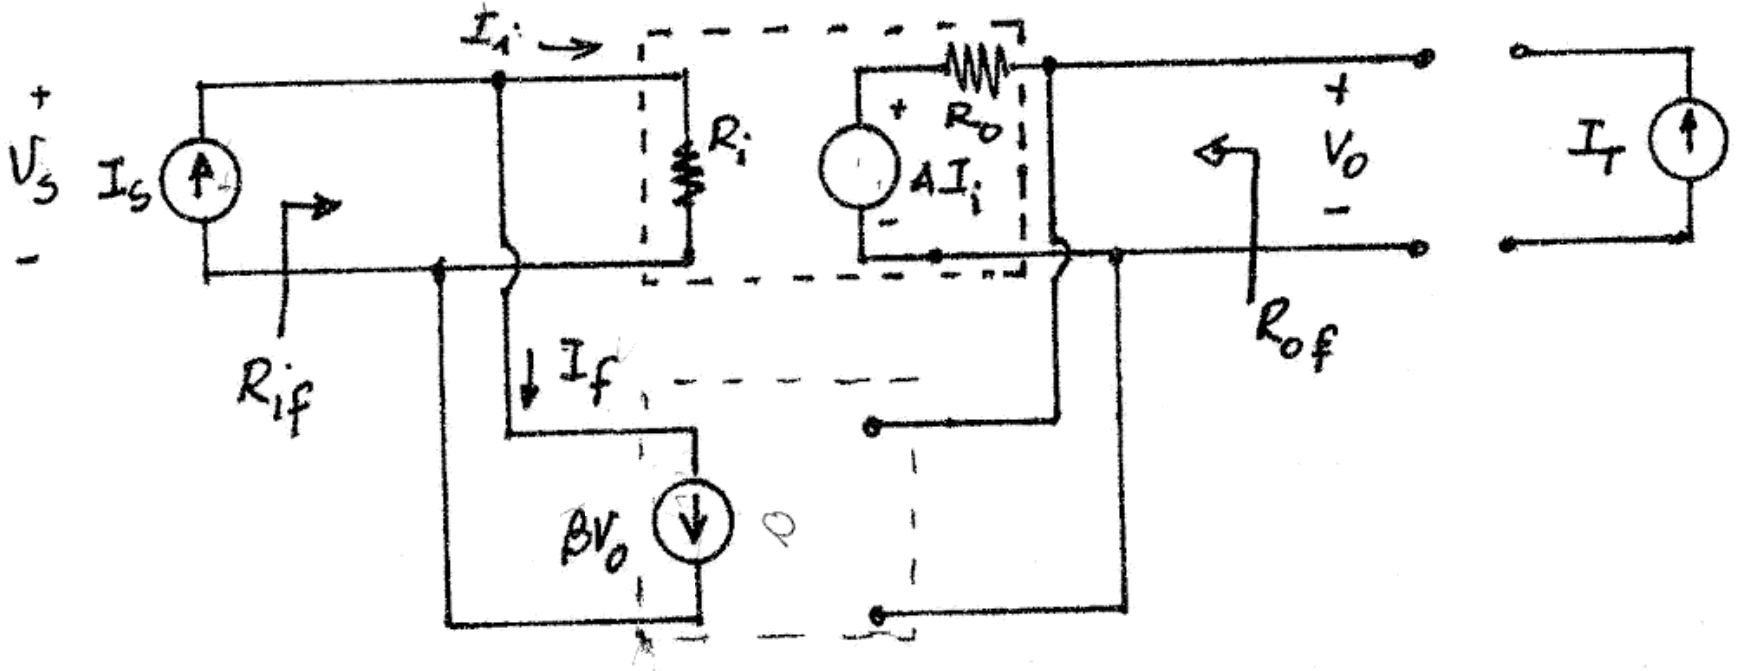
\includegraphics[width=0.9\linewidth]{_fig/retro_m-nodo_c-nodo.png}
	\caption{Muestreo de Nodo - Comparación de Nodo}
	\label{fig:retro_m-nodo_c-nodo}
\end{figure}

La ganancia con retroalimentación, $A_f$, es la relación entre el voltaje de salida y la corriente de entrada: $A_f = V_o / I_s$. Se tiene: \( V_o = A I_i = A (I_s - I_f) = A (I_s - \beta V_o) \) o:

\begin{equation}
	A_f = \frac{V_o}{I_s} = \frac{A}{1 + A\beta}
	\label{equ:retro_ganancia}
\end{equation}

Ésta es la relación clásica de retroalimentación.

La resistencia de entrada con retroalimentación, $R_{if}$, es la resistencia que se ve desde la fuente $I_s$. Se tiene:

\[
R_{if} = \frac{V_s}{I_s} = I_i \frac{R_i}{I_s} = \frac{(I_s - I_f) R_i}{I_s}
\]

\[
R_{if} = \frac{(I_s - \beta V_o) R_i}{I_s} = \frac{(I_s - \beta A I_s)}{(1 + A \beta)} \frac{R_i}{I_s}
\]

\begin{equation}
	R_{if} = \frac{R_i}{1 + A \beta}
	\label{equ:retro_rif}
\end{equation}

Entonces, con comparación de nudo, la resistencia de entrada con retroalimentación es igual a la resistencia de entrada del amplificador sin retroalimentación dividida por el factor $(1 + A \beta)$. Ver por ejemplo la Tabla \ref{tab:retro_comparativo}.

La resistencia de salida con retroalimentación es la resistencia vista desde los terminales de salida. Si inyectamos una fuente de corriente entre los bornes de salida y apagamos la fuente \( I_s \) de entrada, se obtienen los siguientes resultados:

\( V_o = I_T R_o + A I_i\), pero  \(I_i = -I_f = -\beta V_o \)

Entonces: \( V_o (1 + A \beta) = I_T R_o \) ó

\begin{equation}
	R_{of} = \frac{V_o}{I_T} = \frac{R_o}{1 + A \beta}
	\label{equ:retro_rof}
\end{equation}

Con muestreo de nudo, la resistencia de salida con retroalimentación es igual a la resistencia de salida del amplificador sin retroalimentación dividida por el factor \( (1 + A \beta) \). Nuevamente comparar con la Tabla \ref{tab:retro_comparativo}.

El esquema de la Figura \ref{fig:retro_m-nodo_c-nodo} se reduce al esquema de la Figura \ref{fig:retro_m-nodo_c-nodo_equi-reducido} con las equivalencias encontradas.

\begin{figure}[h]
	\centering
	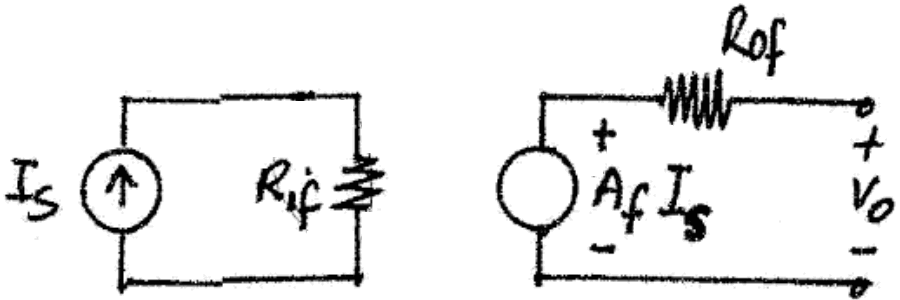
\includegraphics[width=0.7\linewidth]{_fig/retro_m-nodo_c-nodo_equi-reducido.png}
	\caption{Equivalente reducido de diagrama anterior.}
	\label{fig:retro_m-nodo_c-nodo_equi-reducido}
\end{figure}

Ahora lo que queremos es adaptar un circuito real, como el indicado en la Figura 3.40, a este esquema idealizado, para poder aplicar los resultados de las ecuaciones \ref{equ:retro_ganancia}, \ref{equ:retro_rif} y \ref{equ:retro_rof}.

Se reemplazan los bloques funcionales \( A \) y \( \beta \) por el cuadripolo apropiado según el tipo de retroalimentación. Con comparación de nodo, deberíamos escoger el cuadripolo de modo que la fuente y los elementos de entrada del cuadripolo se unan en un par de nodos comunes. De igual forma, con muestreo de nodo, queremos un cuadripolo con un par de nodos comunes a la salida. 

El cuadripolo \( y \), basado en las admitancias de cortocircuito, \( y_i \), \( y_o \), \( y_r \), cumple con estas condiciones. Queda la Figura \ref{fig:retro_m-nodo_c-nodo_cuadripolo}.

\begin{figure}[h]
	\centering
	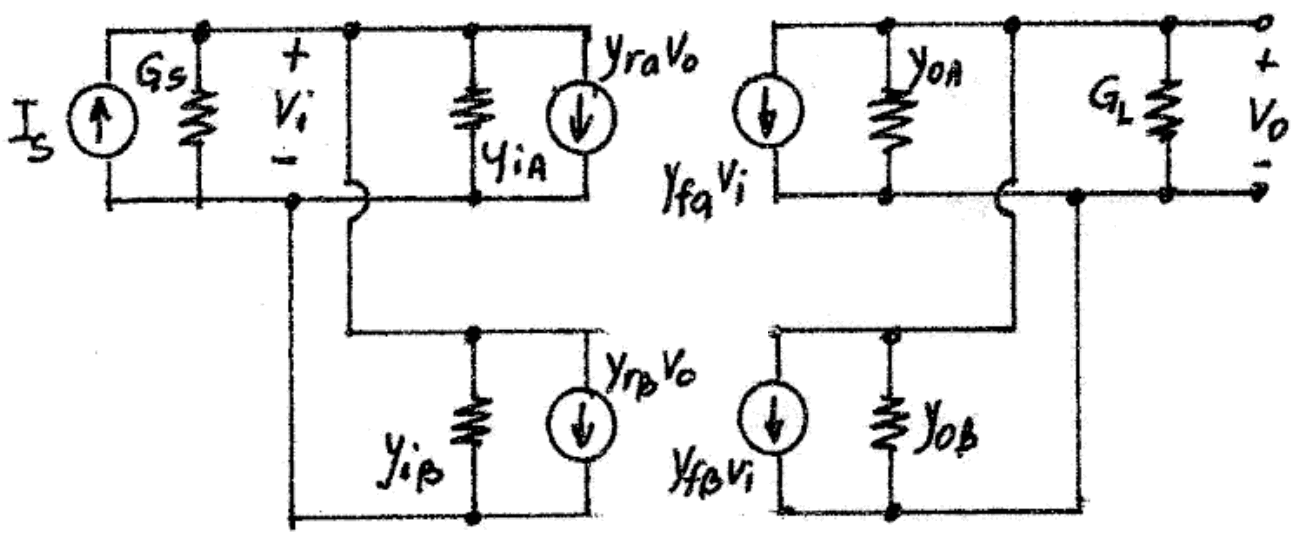
\includegraphics[width=0.9\linewidth]{_fig/retro_m-nodo_c-nodo_cuadripolo.png}
	\caption{Cuadripolo \( y \) aplicado a \( A \) y \( \beta \).}
	\label{fig:retro_m-nodo_c-nodo_cuadripolo}
\end{figure}

Se hace recordar que el cuadripolo \( y \) utiliza las tensiones de entrada y de salida como variables independientes, y las corrientes de entrada y salida como variables dependientes.

\begin{figure}[h]
	\centering
	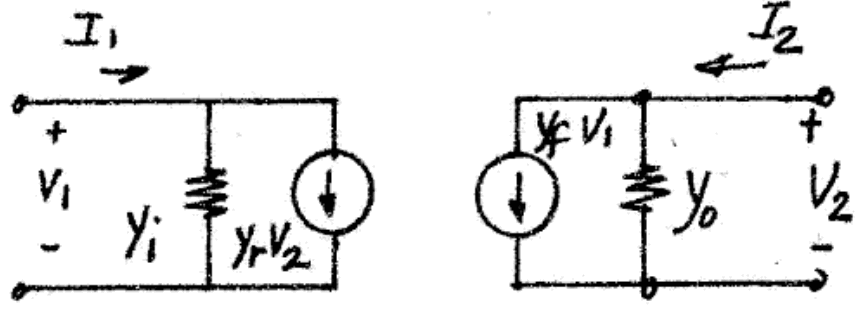
\includegraphics[width=0.9\linewidth]{_fig/retro_m-nodo_c-nodo_cuadripolo-y.png}
	\caption{Cuadripolo \( y \)}
	\label{fig:retro_m-nodo_c-nodo_cuadripolo-y}
\end{figure}			

Según se desprende de la Figura \ref{fig:retro_m-nodo_c-nodo_cuadripolo-y}, se obtiene:

\begin{equation}
	I_1 = y_{i} V_1 + y_{r} V_2
\end{equation}

\begin{equation}
	I_2 = y_{f} V_1 + y_{o} V_2
\end{equation}

donde:

\( y_{i} = \frac{I_{1}}{V_{1}} \) con la salida en cortocircuito, es la admitancia de entrada.

\( y_{r} = \frac{I_{1}}{V_{2}} \) con la entrada en cortocircuito, es la transadmitancia reversa.

\( y_{f} = \frac{I_{2}}{V_{1}} \) con la salida en cortocircuito, es la transadmitancia directa.

\( y_{o} = \frac{I_{2}}{V_{2}} \) con la salida en cortocircuito, es la admitancia de salida.

Volviendo a la Figura \ref{fig:retro_m-nodo_c-nodo_cuadripolo}, se obtiene:

\begin{equation}
	I_{s} = (G_s + Y_{1A} + Y_{1B}) V_{1} + (Y_{rA} + Y_{r \beta}) V_o
\end{equation}

\begin{equation}
	0 = (Y_{fA} + Y_{fB}) V_{1} + (G_{L} + Y_{oA} + Y_{o \beta}) V_o
\end{equation}

Dado que:

\begin{equation}
	Y_{i} = G_{s} + Y_{1A} + Y_{1B}
\end{equation}

\begin{equation}
	Y_{o} = G_{L} + Y_{oA} + Y_{oB}
\end{equation}

Entonces:

\begin{equation}
	\frac{V_o}{I_s} = \frac{-(Y_{fA} + Y_{fB})}{Y_i Y_o - (Y_{rA} + Y_{rB})(Y_{fA} + Y_{fB})}
\end{equation}

Para llevar esta expresión a la forma clásica de la ganancia con retroalimentación, se puede organizar de la siguiente forma:

\begin{equation}
	\frac{V_o}{I_s} = \frac{-(Y_{fA} + Y_{fB}) / Y_i Y_o}{1 - (Y_{rA} + Y_{rB}) / Y_i}
\end{equation}

de donde:

\begin{equation} \label{equ:retro_m-nodo_c-nodo_orig-A}
	A = \frac{-(Y_{fA} + Y_{fB})}{Y_i Y_o}
\end{equation}

y:

\begin{equation} \label{equ:retro_m-nodo_c-nodo_orig-B}
	\beta = Y_{rA} + Y_{rB}
\end{equation}

Para poder interpretar fácilmente estas expresiones, se hacen las siguientes suposiciones, que posteriormente se convertirán en condiciones necesarias para poder aplicar nuestro método:

\textbf{a)} el amplificador da más ganancia en sentido directo que la red de retroalimentación, es decir:

\begin{equation} \label{equ:retro_m-nodo_c-nodo_admitancia-yfA}
	|Y_{fA}| >> |Y_{fB}|
\end{equation}

\textbf{b)} la señal retroalimentada a la entrada de la salida se debe más a la red de retroalimentación que al amplificador, es decir:

\begin{equation} \label{equ:retro_m-nodo_c-nodo_admitancia-yfB}
	|Y_{rA}| << |Y_{rB}|
\end{equation}

\textbf{c)} la admitancia de salida no afecta mucho la admitancia de entrada, es decir:

\begin{equation} \label{equ:retro_m-nodo_c-nodo_admitancias}
	|Y_{fA} Y_{rA}| << |Y_i Y_o|
\end{equation}

Entonces la expresión \ref{equ:retro_m-nodo_c-nodo_orig-A} se convierte en la siguiente:

\[ A = -Y_{fA} / Y_i Y_o \]

\begin{equation} \label{equ:retro_m-nodo_c-nodo_A}
	A = -Y_{fA} / (G_s + Y_{iA} + Y_{iB}) (G_L + Y_{oA} + Y_{oB})
\end{equation}

donde se destaca la presencia de componentes de la red $\beta$. Y la expresión \ref{equ:retro_m-nodo_c-nodo_orig-B} se convierte en:

\begin{equation} \label{equ:retro_m-nodo_c-nodo_B}
	\beta \cong Y_{rB}
\end{equation}

que depende solo de la red $\beta$.

\begin{figure}[h]
	\centering
	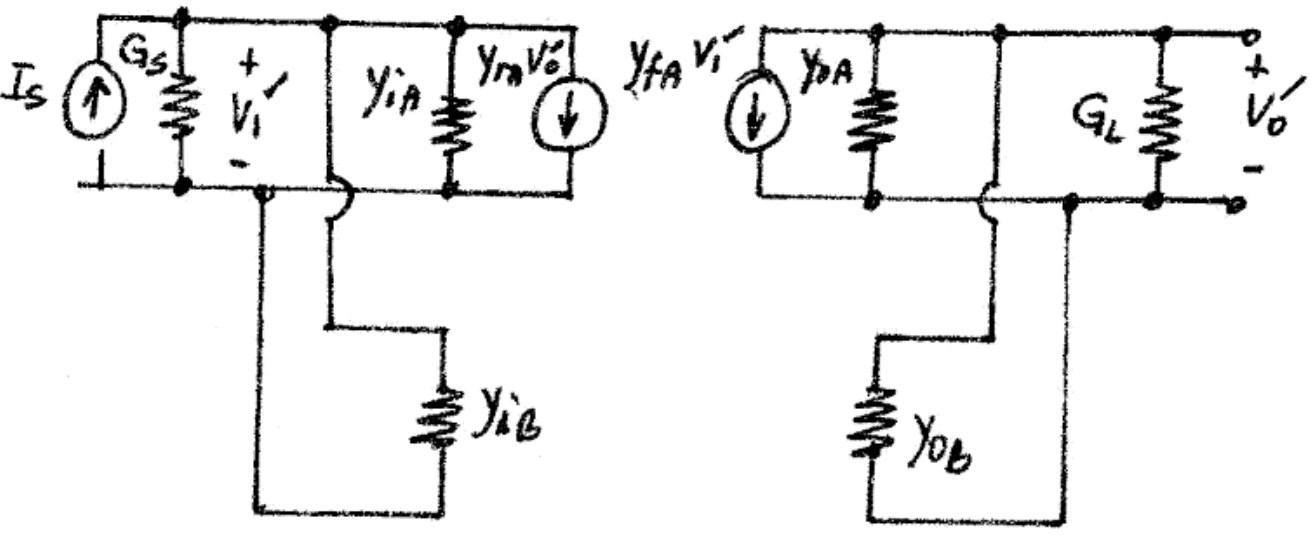
\includegraphics[width=0.9\linewidth]{_fig/retro_m-nodo_c-nodo_hallar-a.png}
	\caption{Circuito para hallar \( A = \frac{V_o}{I_s} \)}
	\label{fig:retro_m-nodo_c-nodo_hallar-a}
\end{figure}			

La expresión \ref{equ:retro_m-nodo_c-nodo_A} para A tiene una interpretación circuital muy interesante que se indica en la Figura \ref{fig:retro_m-nodo_c-nodo_hallar-a}. De este circuito se consigue:

\begin{equation} \label{equ:retro_m-nodo_c-nodo_solve-A}
	A = V_o^{\prime} / I_s = -Y_{fA} / (Y_i Y_o - Y_{fA} Y_{rA})
\end{equation}

\begin{figure}[h]
	\centering
	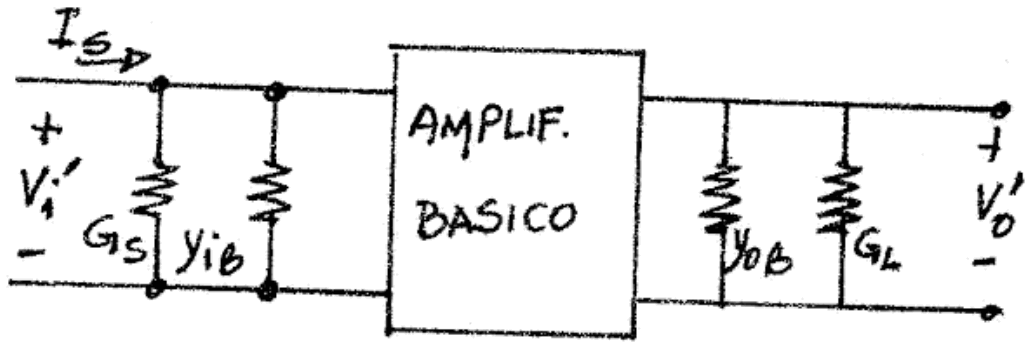
\includegraphics[width=0.9\linewidth]{_fig/retro_m-nodo_c-nodo_solve-hallar-a.png}
	\caption{Circuito para hallar \( A \) compacto}
	\label{fig:retro_m-nodo_c-nodo_solve-a}
\end{figure}

pero si es aplicable la desigualdad \ref{equ:retro_m-nodo_c-nodo_admitancias} entonces la ecuación \ref{equ:retro_m-nodo_c-nodo_solve-A} se reduce a la ecuación \ref{equ:retro_m-nodo_c-nodo_A}. ¿Y cual es el circuito de la Figura \ref{fig:retro_m-nodo_c-nodo_hallar-a}? Es el circuito original con la retroalimentación eliminada, pero con el efecto de carga de la red de retroalimentación incluido, tal como se aprecia más claramente en la Figura \ref{fig:retro_m-nodo_c-nodo_solve-a}. Es decir, nos queda la fuente de entrada con su resistencia, la salida con su resistencia de carga, el amplificador completo, a la entrada se anexa $Y_{iB}$, la admitancia de entrada de la red de retroalimentación con la salida en cortocircuito, y a la salida se anexa \( Y_{oB} \), la admitancia de salida de la red de retroalimentación con la entrada en cortocircuito. Al finalizar esta sección resolveremos ejemplos donde se aplicará este análisis.

En cuanto a la retroalimentación, con la aplicación de las desigualdades, nos queda:

\begin{equation}
	\beta = Y_{rB}
\end{equation}

\begin{figure}[h]
	\centering
	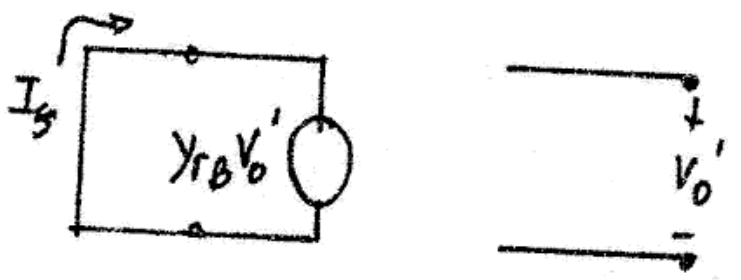
\includegraphics[width=0.9\linewidth]{_fig/retro_m-nodo_c-nodo_admitancia-reversa.png}
	\caption{Admitancia reversa}
	\label{fig:retro_m-nodo_c-nodo_admitancia-reversa}
\end{figure}

la admitancia reversa de la red de retroalimentación, que se encuentra como la relación de la corriente de retroalimentación a la tensión de salida con la entrada en cortocircuito, como se indica en la Figura \ref{fig:retro_m-nodo_c-nodo_admitancia-reversa}.

Antes de seguir con los ejemplos, vamos a demostrar el efecto de la retroalimentación sobre las admitancias de entrada y salida para el caso de Muestreo de Nodo - Comparación de Nodo.

\begin{figure}[h]
	\centering
	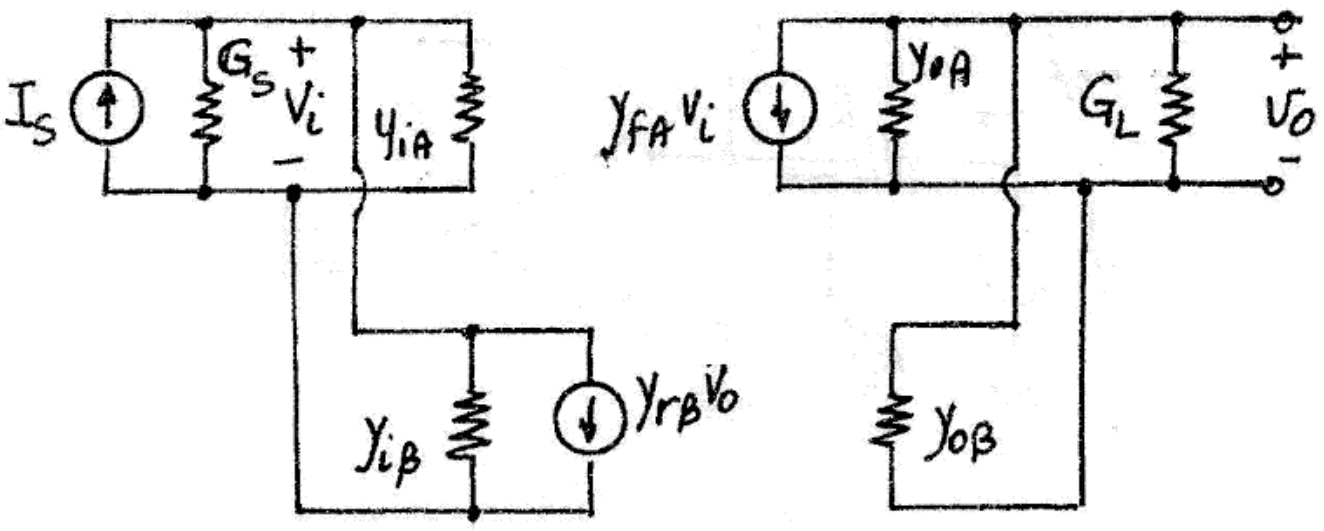
\includegraphics[width=0.9\linewidth]{_fig/retro_m-nodo_c-nodo_admitancia-entrada.png}
	\caption{Admitancia de entrada}
	\label{fig:retro_m-nodo_c-nodo_admitancia-entrada}
\end{figure}

En la Figura \ref{fig:retro_m-nodo_c-nodo_admitancia-entrada}, se busca la admitancia de entrada con el modelo general, donde se ignora \( Y_{fB} A \) y \( Y_{rA} \) por considerarlos despreciables, según la discusión anterior. Nos queda:

\begin{equation}
	I_s = V_i (G_s + Y_{iA} + Y_{iB}) + Y_{rB} V_o
\end{equation}

e,

\begin{equation}
	( Y_{oA}  + G_L + Y_{oB} ) = -Y_{fA} V_i
\end{equation}

ó, $ V_o = -(\frac{Y_{fA}}{Y_o} V_i $, de donde $ I_s = V_i (Y_i - \frac{Y_{fA}Y_{rB}}{Y_o} ) = V_i ( Y_i ( 1 - \frac{Y_{fA}}{Y_i Y_{o}} ) Y_{rB}) $ ó

\begin{equation}
	\frac{I_s}{V_i} = Y_i (1 + A\beta).
\end{equation}

es decir, la admitancia de entrada aumenta por el factor \( 1 + A\beta \); la resistencia de entrada se reduce por \( 1 + A\beta \).

En la Figura \ref{fig:retro_m-nodo_c-nodo_sch-ext}, se muestra el circuito a analizar para hallar la admitancia en los nodos de salida. Entonces:

\begin{equation}
	I_T = V_o (G_L + y_{oA} + y_{oB}) + y_{fA} V_i 
\end{equation}

\begin{equation}
	V_i (G_s + y_{iA} + y_{iB}) = -y_{fB} V_o
\end{equation}

o,

\[
V_i = -\left( \frac{y_{fB}}{G_s + y_{iA} + y_{iB}} \right) V_o
\]

Luego,

\begin{equation}
	I_T = V_o \left( G_L + y_{oA} + y_{oB} - y_{fA} \frac{y_{fB}}{G_s + y_{iA} + y_{iB}} \right)
\end{equation}

o bien,

\begin{equation}
	\frac{I_T}{V_o} = G_L + y_{oA} + y_{oB} - \frac{y_{fA} y_{fB}}{G_s + y_{iA} + y_{iB}}
\end{equation}

es decir, la admitancia de salida aumenta por el factor $1 + AB$.

\begin{figure}[h]
	\centering
	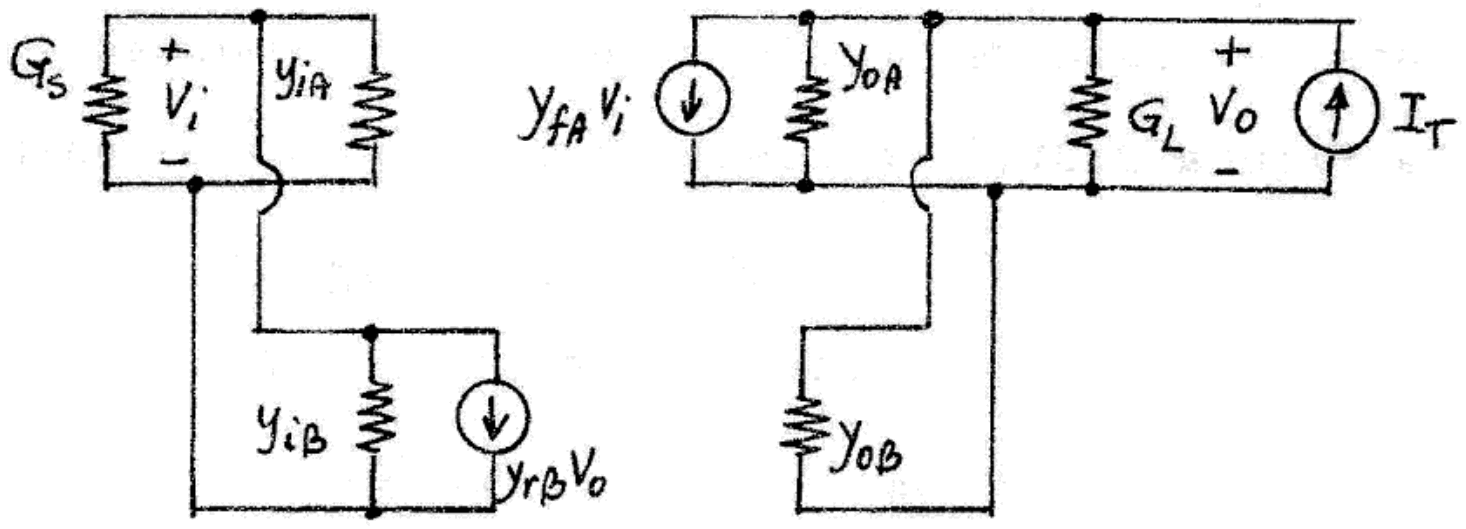
\includegraphics[width=0.8\linewidth]{_fig/retro_m-nodo_c-nodo_sch-ext.png}
	\caption{Circuito equivalente para hallar admitancia}
	\label{fig:retro_m-nodo_c-nodo_sch-ext}
\end{figure}

Ahora, vamos a resolver un par de ejemplos para demostrar la aplicación de la teoría que se acaba de describir.

\subsubsection{Ejemplo A} %p152

En la Figura \ref{fig:retro_m-nodo_c-nodo_ejm1a} se muestra un amplificador con retroalimentación.

\begin{figure}[h]
	\centering
	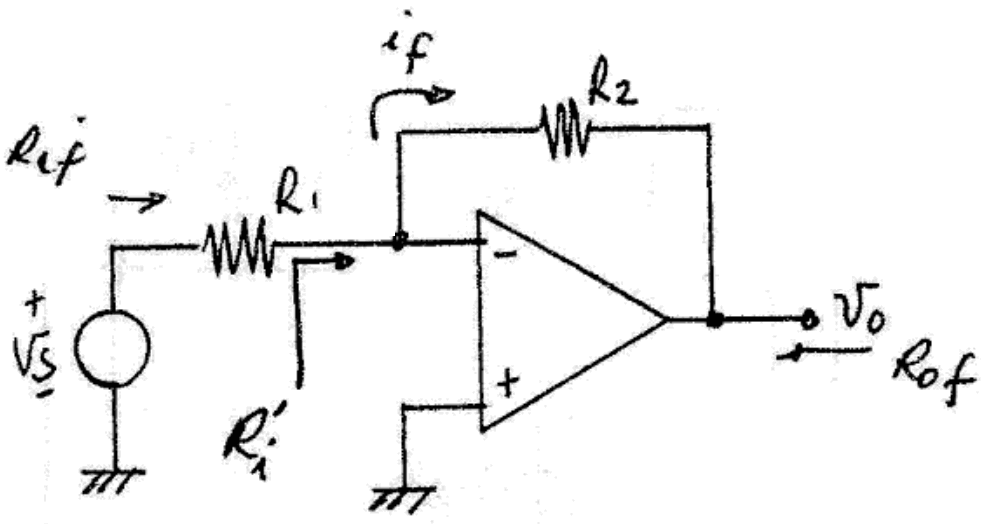
\includegraphics[width=0.6\linewidth]{_fig/retro_m-nodo_c-nodo_ejm1a.png}
	\caption{Ejemplo: Circuito amplificador con retroalimentación}
	\label{fig:retro_m-nodo_c-nodo_ejm1a}
\end{figure}

Lo \textbf{Primero} que hace falta es identificar el tipo de retroalimentación: la retroalimentación se crea por medio de la rama \( R_2 \). Esta rama llega al mismo nodo de entrada, y por lo tanto es comparación de nodo. En la salida, se toma la señal de retroalimentación en el nodo de salida, por lo tanto es muestreo de nodo, es decir, se muestra la tensión de salida.

Lo \textbf{Segundo} es hallar el punto de operación. Con los operacionales este paso no es necesario ya que la polarización consiste sencillamente en conectar las fuentes de DC.

\textbf{Tercero}, se crea el amplificador \( A \) en lazo abierto. Se elimina la red de retroalimentación para dejar el amplificador sin retroalimentación, al cual se anexa a la entrada y a la salida el efecto de carga de la red de retroalimentación siguiendo los pasos previamente establecidos. El resultado se muestra en la Figura \ref{fig:retro_m-nodo_c-nodo_ejm1b}.

\begin{figure}[h]
	\centering
	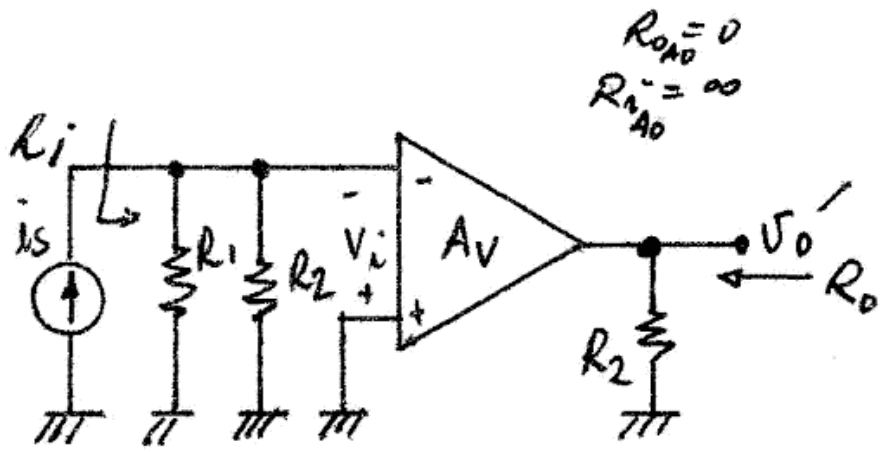
\includegraphics[width=0.6\linewidth]{_fig/retro_m-nodo_c-nodo_ejm1b.png}
	\caption{Circuito amplificador con retroalimentación}
	\label{fig:retro_m-nodo_c-nodo_ejm1b}
\end{figure}

Nuevamente hemos convertido la fuente de entrada, junto con su resistencia, en el equivalente de Norton por considerarse de una retroalimentación tipo comparación de nodo. De aquí se obtiene:

\[
A = \frac{v_o'}{i_s} = -A_V (R_1 || R_2)
\]

\[
R_i = R_1 || R_2
\]

\[
R_o = 0
\]

y la respuesta de frecuencia sin retroalimentación.

\textbf{Cuarto}, se encuentra \( \beta \). La red de retroalimentación está formada por \( R_2 \).  \( \beta \) viene dada por \( \frac{i_f}{v_o} \) con la entrada en cortocircuito, o \( \frac{i_f}{v_o} = \frac{-1}{R_2} \)

Próximamente, dado los valores sin retroalimentación, y \( \beta \), se determinan las características del circuito con retroalimentación. Tenemos:

\[
D = 1 + A\beta = 1 + A_V R_1 / (R_1 + R_2)
\]

\[
A_f = A / D = -A_V (R_1 || R_2) / \left(1 + A_V R_1 / (R_1 + R_2)\right)
\]

\[
R_{if} = R_i / D = R_1 || R_2 / \left(1 + A_V R_1 / (R_1 + R_2)\right)
\]

\[
R_{of} = R_o / D = 0
\]

\[
\frac{v_o}{v_s} = v_o (i_s R) = \frac{A_f}{R_i} = -\frac{R_2}{R_1} \frac{1}{1 + (1 + R_2 / R_1) / A_V}
\]

Finalmente encontramos de nuevo la resistencia de entrada por medio de esta técnica de retroalimentación que se encontró previamente "a pie". Así:

\[
R_i' = \frac{1}{\left( \frac{1}{R_{if}} - \frac{1}{R_1} \right)} = \frac{R_2}{1 + A_V}
\]

\subsubsection{Ejemplo B} %p154

En la Figura \ref{fig:retro_m-nodo_c-nodo_ejm2a} se muestra un amplificador con retroalimentación.

\begin{figure}[h]
	\centering
	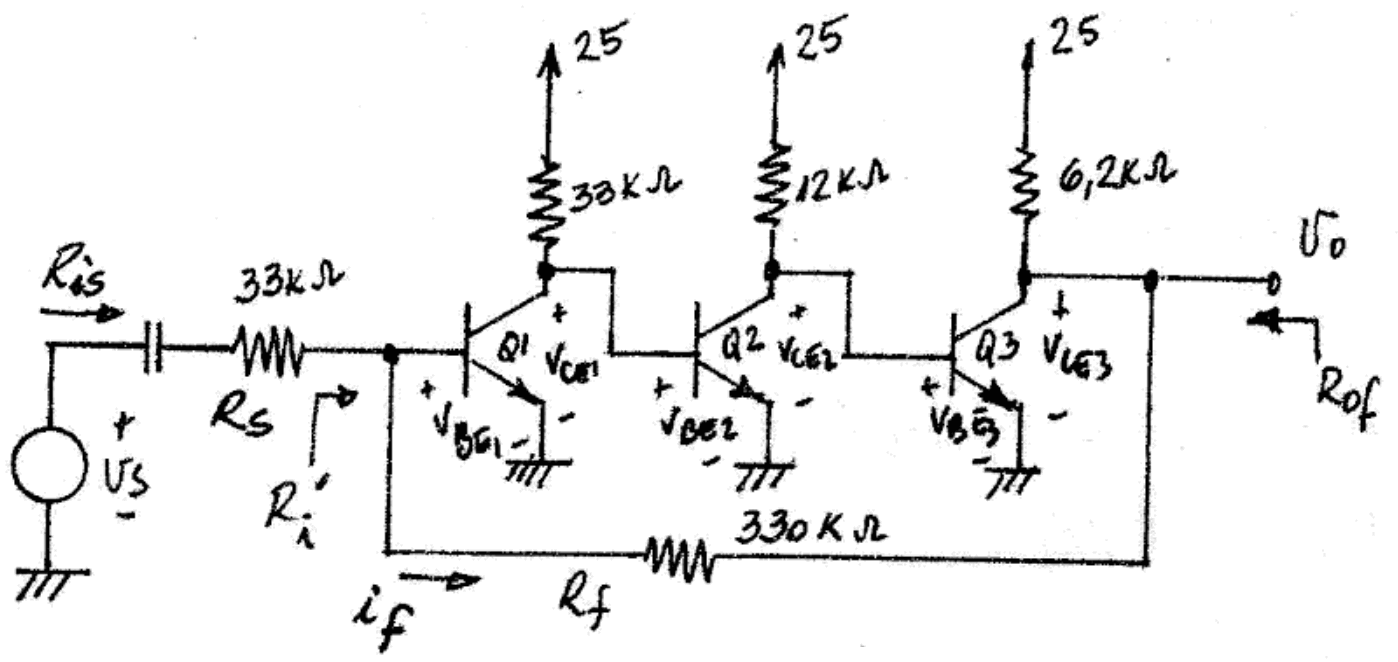
\includegraphics[width=0.8\linewidth]{_fig/retro_m-nodo_c-nodo_ejm2a.png}
	\caption{Ejemplo}
	\label{fig:retro_m-nodo_c-nodo_ejm2a}
\end{figure}

\textbf{Primero:} Identificación del tipo de retroalimentación: la retroalimentación se crea por medio de la rama \( R_f \). Esta rama llega al mismo nodo de entrada, y por lo tanto es comparación de nodo. En la salida, se toma la señal de retroalimentación en el nodo de salida, por lo tanto es muestreo de nodo, es decir se muestrea la tensión de salida.

\textbf{Segundo:} Hallar el punto de operación. En continua queda el circuito que se muestra en la Figura \ref{fig:retro_m-nodo_c-nodo_ejm2b}.

\begin{figure}[h]
	\centering
	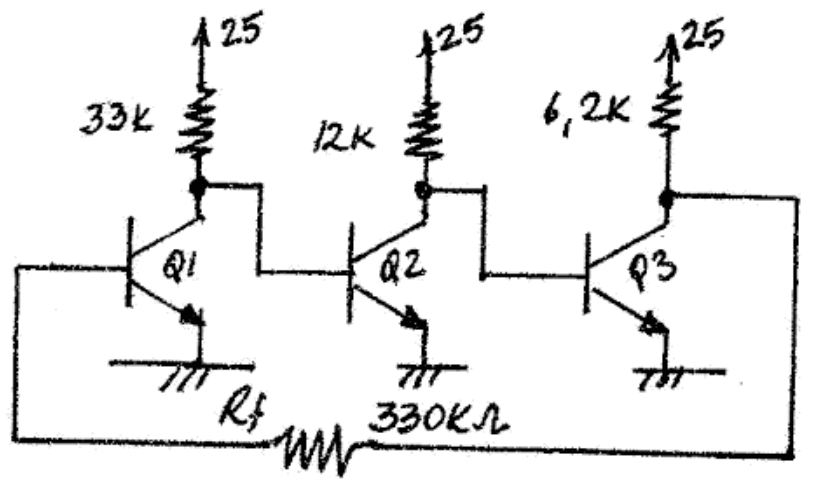
\includegraphics[width=0.7\linewidth]{_fig/retro_m-nodo_c-nodo_ejm2b.png}
	\caption{Circuito en dc de la Figura \ref{fig:retro_m-nodo_c-nodo_ejm2a}}
	\label{fig:retro_m-nodo_c-nodo_ejm2b}
\end{figure}

Primero se hace la observación que la misma tensión base-emisor es el voltaje colector-emisor de la etapa anterior, al menos en el acople del primer transistor con el segundo, y del segundo transistor con el tercero. Entonces

\[ V_{CE1} = V_{BE2} = 0.7V \]

\[ V_{CE2} = U_{BE3} = 0.7V \]

Ambos resultados nos garantizan \( V_{CE} > V_{CE(sat)} = 0.2V \) por lo que estamos fuera de la región de saturación. De aquí podemos calcular las corrientes de colector de los primeros dos transistores:

\[ I_{C1} \approx \frac{25 - 0.7}{33K} = 0.74 mA \]

\[ I_{C2} \approx \frac{25 - 0.7}{12K} = 2.02 mA \]

Para \( Q3 \) nos queda:

\[ 25 = I_{C3} \cdot 6.2K + I_{B1} \cdot 330K + 0.7 \]

De donde:

\[ I_{C3} = 3.5 mA \]

\[ V_{CE3} = 3.2 V \]

\textbf{Tercero:} Con estos valores de los puntos de operación se calculan los valores de los parámetros de los transistores:

\begin{tabular}{ccc}
	\( q_{m1} = 0.0285 \) & \( q_{m2} = 0.0777 \) & \( q_{m3} = 0.135 \) \\
	\( r_{\pi1} = 3513 \) & \( r_{\pi2} = 1287 \) & \( r_{\pi3} = 748 \) \\
\end{tabular}

\begin{figure}[h]
	\centering
	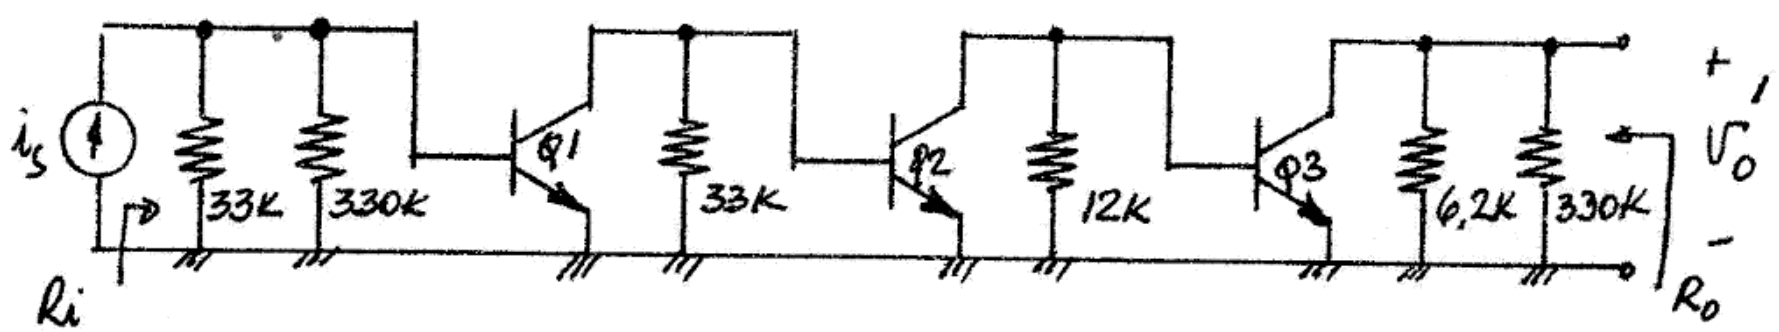
\includegraphics[width=0.8\linewidth]{_fig/retro_m-nodo_c-nodo_ejm2c.png}
	\caption{Circuito sin Retroalimentación, parte A}
	\label{fig:retro_m-nodo_c-nodo_ejm2c}
\end{figure}
\begin{figure}[h]
	\centering
	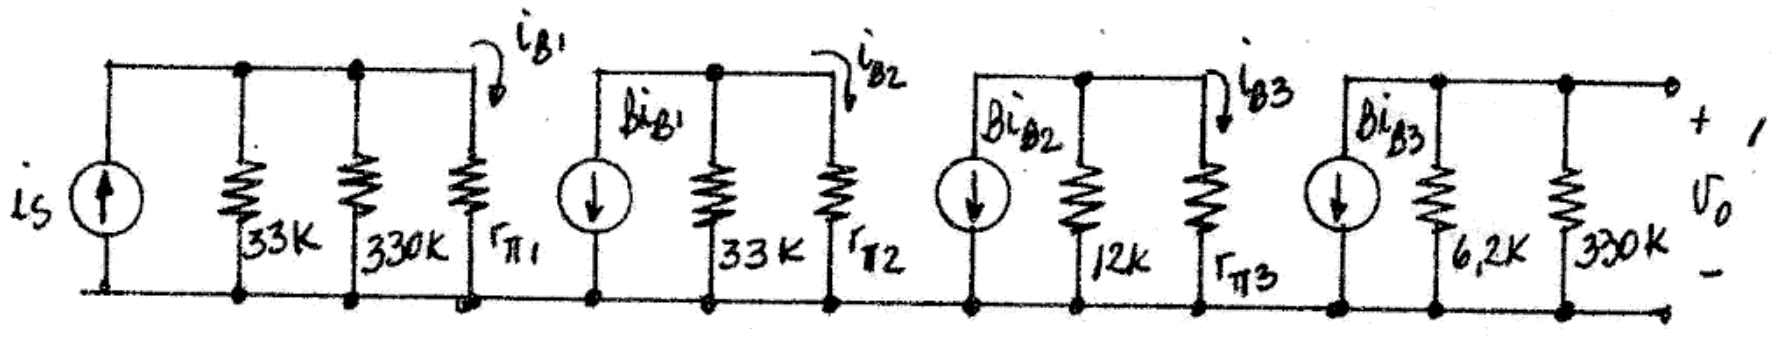
\includegraphics[width=0.8\linewidth]{_fig/retro_m-nodo_c-nodo_ejm2d.png}
	\caption{Circuito sin Retroalimentación, parte B}
	\label{fig:retro_m-nodo_c-nodo_ejm2d}
\end{figure}

Se elimina la red de retroalimentación para dejar el amplificador sin retroalimentación, al cual se anexa a la entrada y a la salida el efecto de carga de la red de retroalimentación. El resultado se muestra en la Figura \ref{fig:retro_m-nodo_c-nodo_ejm2c}, con su circuito equivalente a frecuencias medidas en la Figura \ref{fig:retro_m-nodo_c-nodo_ejm2d}.

Se hace notar que hemos convertido la fuente de entrada, junto con su resistencia, en el equivalente de Norton por considerarse de una retroalimentación tipo comparación de nodo. De aquí procedemos normalmente para obtener:

\[ A = \frac{i_o\prime\prime}{i_s} = -503 \]

\[ R_i = 1785 \]

\[ R_o = \infty \]

De querer la respuesta de frecuencia sin retroalimentación se volverían a colocar los condensadores, y se trabajaría con el modelo de alta frecuencia del transistor.

\textbf{Cuarto:} La red de retroalimentación está formada por $R_f$. $\beta$ viene dada por: $\frac{i_s}{v_o} = -\frac{1}{R_f}$

\textbf{Quinto:} Dados los valores sin retroalimentación, \( A \) y \( \beta \), se determinan las características del circuito con retroalimentación. Tenemos:

\[ D = 1 + A\beta = 14962 \]

\[ A_f = \frac{A}{D} = -329978 \Omega \]

\[ R_{if} = \frac{R_i}{D} = 0.21 \Omega	\]

\[ R_{of} = \frac{R_o}{D} = 0.41 \Omega	\]

\[ \frac{v_o}{v_s} = \frac{v_o}{(i_s R_s)} = \frac{A_f}{R} = -9.9993 \approx -10 \]

Finalmente, encontramos resistencias de entrada. Así:

\[ R_i' = \left( \frac{1}{R_{if}} - \frac{1}{R_s} \right)^{-1} = 0.21 \Omega \]

\[ R_{is} = R_s + R_i' \approx R_s = 33 k\Omega	\]

De esta forma, hemos analizado a fondo la metodología de retroalimentación aplicada al caso \textbf{Muestreo de Nodo - Comparación de Nodo}. A continuación, se tratan los otros casos de retroalimentación. El análisis es muy parecido, lo que permitirá acortar un poco su presentación.

\subsection{Muestreo de Lazo - Comparación de Lazo} %p157

\begin{figure}[h]
	\centering
	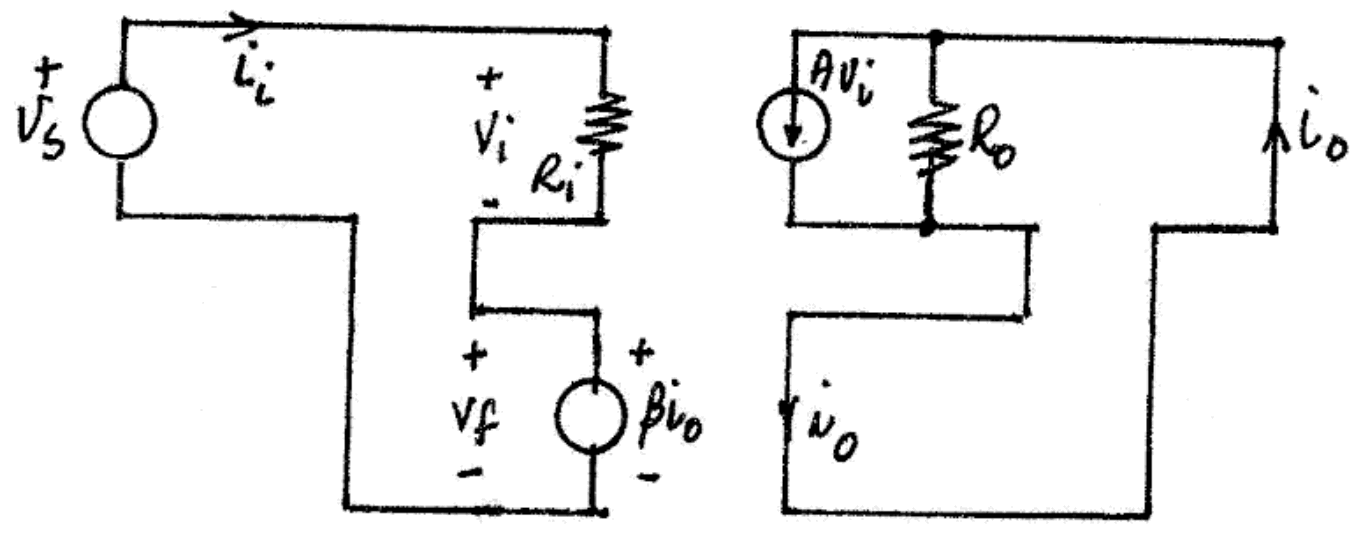
\includegraphics[width=0.8\linewidth]{_fig/retro_m-lazo_c-lazo.png}
	\caption{Muestreo de Lazo - Comparación de Lazo}
	\label{fig:retro_m-lazo_c-lazo}
\end{figure}

En la Figura \ref{fig:retro_m-lazo_c-lazo}, tenemos el diagrama idealizado de la retroalimentación tipo \textbf{Muestreo de Lazo - Comparación de Lazo}.

De la figura se obtienen las siguientes relaciones:

\textbf{Ganancia:}

\[ A_f = \frac{i_o}{v_s} \]

\[ i_o = A v_i \]

\[ v_i = v_s - v_f = v_s - \beta i_o \]

\[ i_o = A (v_s - \beta i_o) \]

\[ i_o (1 + A \beta) = A v_s \]

\[ A_f = \frac{i_o}{v_s} = \frac{A}{(1 + A \beta)} \]

\textbf{Resistencia de Entrada;}

\[ R_{if} = \frac{v_s}{i_i}	\]

\[ R_i = \frac{v_i}{i_i} \]

\[ v_s = i_i R_i + \beta i_o = i_I R_i + \frac{\beta A v_s}{1 + A \beta)} \]

\[ v_s \frac{1 - \beta A}{1 + A \beta} = i_i R_i \]

o

\[ R_{if} = \frac{v_s}{i_i} = R_i (1 + A \beta)	\]

Es decir, la resistencia del lazo de entrada aumenta por \( (1 + A \beta) \).

\textbf{Resistencia del Lazo de Salida:}

\begin{equation} \label{retro_m-lazo_c-lazo_rof}
	R_{of} = \frac{v_T}{I_T}
\end{equation}

\begin{figure}[h]
	\centering
	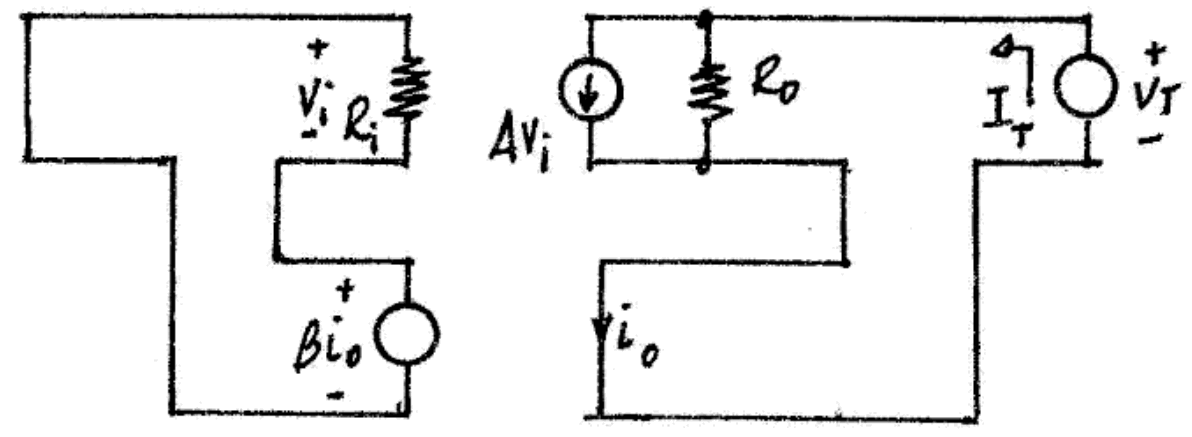
\includegraphics[width=0.8\linewidth]{_fig/retro_m-lazo_c-lazo_analisis-r.png}
	\caption{Muestreo de Lazo - Comparación de Lazo, análisis \( Rof \)}
	\label{fig:retro_m-lazo_c-lazo_analisis-r}
\end{figure}

Ecuacion \ref{retro_m-lazo_c-lazo_rof} según Figura \ref{fig:retro_m-lazo_c-lazo_analisis-r}

Donde:

\[ I_T = A v_i + \frac{v_T}{R_o} \]

\[ v_i = -\beta i_o = -\beta I_T \]

\[ I_T = -\beta A I_T + \frac{v_T}{R_o} \]

o:

\[ I_T (1 + A \beta) = \frac{v_T}{R_o} \]

y:

\[ R_{of} = \frac{v_T}{I_T} = Ro (1 + A \beta) \]

La resistencia del lazo de salida aumenta por \( (1 + A \beta) \). Cuando hablamos de la resistencia del lazo, eso implica abrir el lazo y determinar la resistencia desde el punto abierto, lo que normalmente conlleva a sumar las resistencia en el lazo.

En la figura \ref{fig:retro_m-lazo_c-lazo_a} se traza nuevamente el diagrama de bloques general de Muestreo de Lazo - Comparación de Lazo.

Se reemplaza los bloques funcionales de $A$ y $\beta$ por el cuadripolo apropiado según el tipo de retroalimentación. Con comparación de lazo deberíamos escoger el cuadripolo de modo que la fuente y los elementos de entrada del cuadripolo compartan un lazo común. De igual forma con muestreo de lazo queremos un lazo común a la salida. El cuadripolo $"z"$, basado en las impedancias de circuito abierto, $z_i$, $z_r$, $z_f$, $z_o$ cumple con éstas condiciones. Queda la figura \ref{fig:retro_m-lazo_c-lazo_modelo-cuadripolo-z}.

\begin{figure}[h]
	\centering
	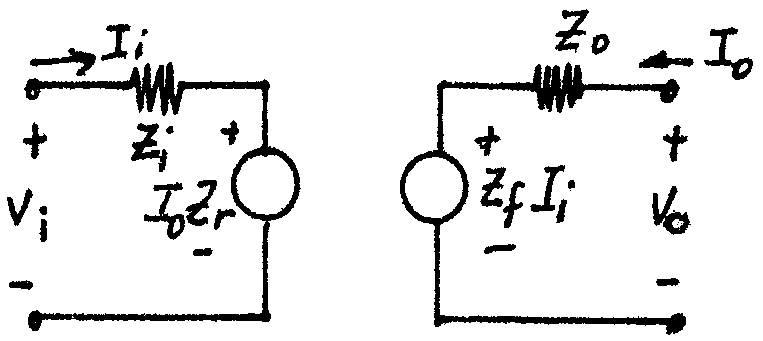
\includegraphics[width=0.6\linewidth]{_fig/retro_m-lazo_c-lazo_modelo-cuadripolo-z.png}
	\caption{Cuadripolo "z"}
	\label{fig:retro_m-lazo_c-lazo_modelo-cuadripolo-z}
\end{figure}

El cuadripolo \( Z \) utiliza las corrientes de entrada y de salida como variables independientes, y las tensiones de entrada y salida como variables dependientes. Se obtiene:

\begin{equation}
	Vi = I_i Z_i + I_o Z_r
\end{equation}			

\begin{equation}
	Vo = I_i Z_f + I_o Z_o
\end{equation}			

Nos queda el modelo de cuadripolos de Muestreo de Lazo - Comparación de Lazo en la Figura \ref{fig:retro_m-lazo_c-lazo_modelo-cuadripolo}.

\begin{figure}[h]
	\centering
	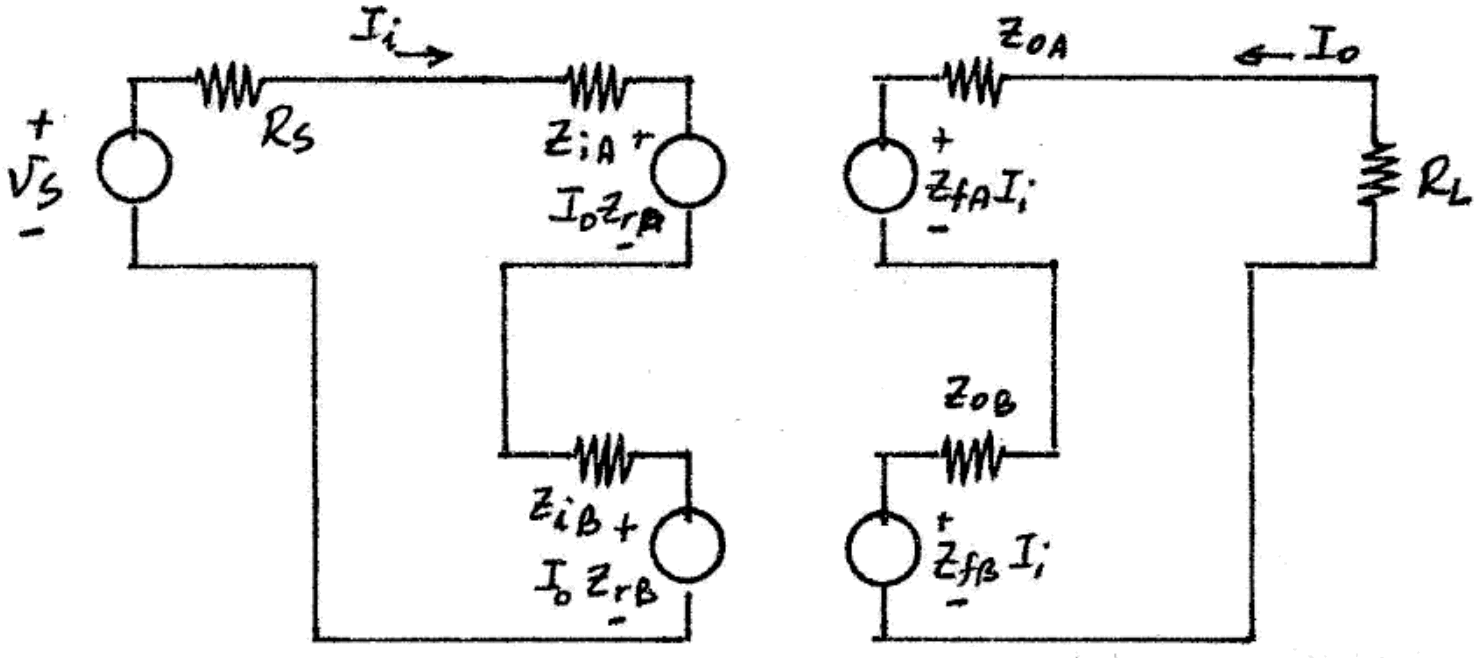
\includegraphics[width=0.8\linewidth]{_fig/retro_m-lazo_c-lazo_modelo-cuadripolo.png}
	\caption{Muestreo de Lazo - Comparación de Lazo}
	\label{fig:retro_m-lazo_c-lazo_modelo-cuadripolo}
\end{figure}

Procediendo como en el caso anterior, si se cumplen las siguientes condiciones: \( |Z_{fA}| \gg |Z_{fB}| \) , \( |Z_{oB}| \gg |Z_{oA}| \) , y \( |Z_{fA} Z_{rA}| \ll |Z_i Z_o| \) , entonces se puede aplicar la Metodología de Retroalimentación, y hallar \( A \) y \( \beta \) por separado.

El circuito de \( A \), el amplificador sin retroalimentación, se muestra en la Figura \ref{fig:retro_m-lazo_c-lazo_hallar-a}, donde se aprecia el anexo de \(Z_{i\beta}\) a la entrada y \(Z_{o\beta}\) a la salida. Se hace notar que \(Z_{i\beta}\) es la impedancia de entrada del circuito de retroalimentación con el lazo de salida abierto, mientras que \(Z_{o\beta}\) es la impedancia de salida del circuito de retroalimentación con el lazo de entrada abierto.

\begin{figure}[h]
	\centering
	\subfloat[Amplificador sin retroalimentación]
	{
		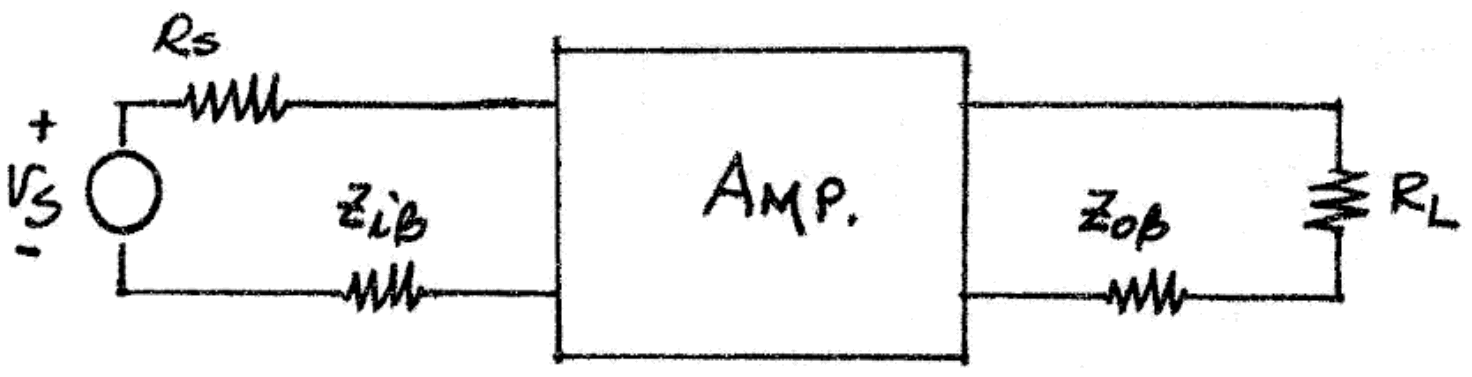
\includegraphics[width=0.44\linewidth]{_fig/retro_m-lazo_c-lazo_hallar-a.png}
		\label{fig:retro_m-lazo_c-lazo_hallar-a}
	}
	\subfloat[Definición de \(\beta\)]
	{
		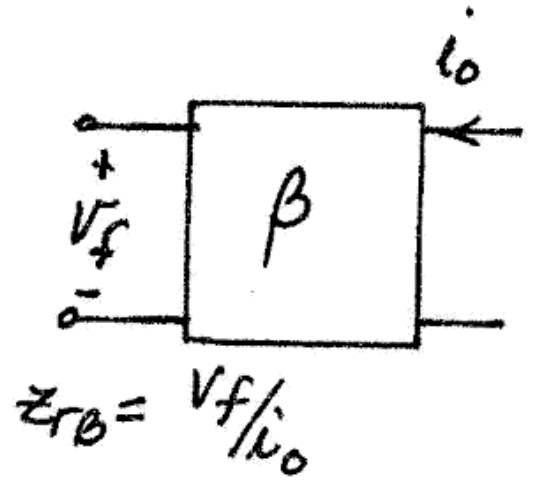
\includegraphics[width=0.44\linewidth]{_fig/retro_m-lazo_c-lazo_hallar-beta.png}
		\label{fig:retro_m-lazo_c-lazo_hallar-beta}
	}
	\caption{Formas para hallar \( A \) y \( \beta \)}
	\label{fig:retro_m-lazo_c-nodo_a-beta}
\end{figure}				

En la Figura \ref{fig:retro_m-lazo_c-lazo_hallar-beta}, el circuito para hallar \( \beta = Z_{o\beta}\), como la relación del voltaje a la entrada a \(V_s\) corriente de salida de la red de retroalimentación, con la entrada abierta.

\subsubsection{Ejemplo}

En las Figuras \ref{fig:retro_m-lazo_c-lazo_ejm-a} y \ref{fig:retro_m-lazo_c-lazo_ejm-b} se muestra un ejemplo de este tipo de retroalimentación. En la Figura \ref{fig:retro_m-lazo_c-lazo_ejm-b} se muestra cómo queda el amplificador sin retroalimentación, en la Figura \ref{fig:retro_m-lazo_c-lazo_ejm-c} la red de retroalimentación.

\begin{figure}[h]
	\centering
	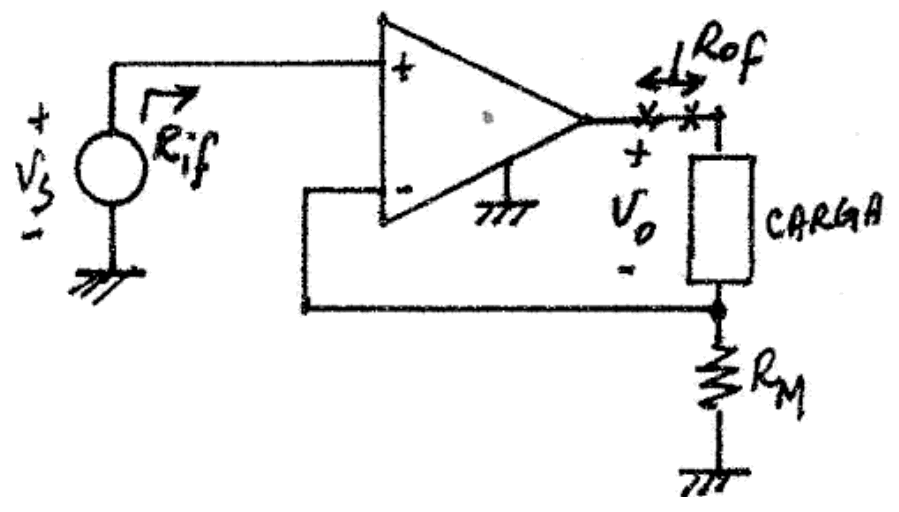
\includegraphics[width=0.8\linewidth]{_fig/retro_m-lazo_c-lazo_ejm-a.png}
	\caption{Ejemplos de retroalimentación: Amplificador}
	\label{fig:retro_m-lazo_c-lazo_ejm-a}
\end{figure}

\begin{figure}[h]
	\centering
	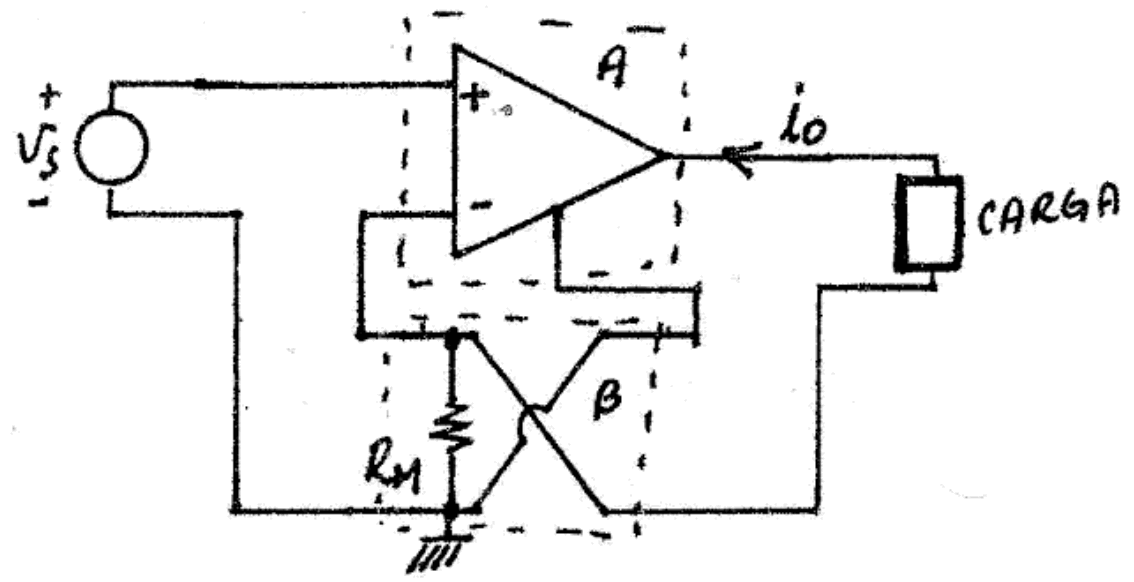
\includegraphics[width=0.8\linewidth]{_fig/retro_m-lazo_c-lazo_ejm-b.png}
	\caption{Ejemplos de retroalimentación: (b) Representación en cuadripolos}
	\label{fig:retro_m-lazo_c-lazo_ejm-b}
\end{figure}

\begin{figure}[h]
	\centering
	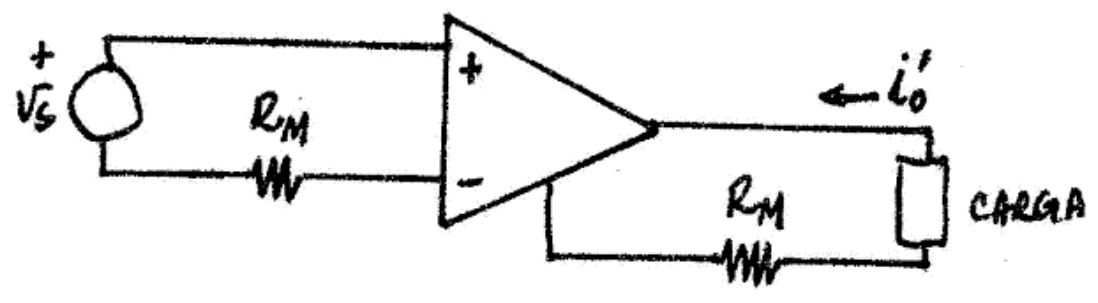
\includegraphics[width=0.6\linewidth]{_fig/retro_m-lazo_c-lazo_ejm-c.png}
	\caption{Ejemplos de retroalimentación: Amplificador sin retroalimentación}
	\label{fig:retro_m-lazo_c-lazo_ejm-c}
\end{figure}

\begin{figure}[h]
	\centering
	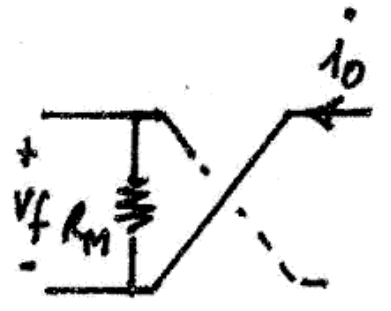
\includegraphics[width=0.3\linewidth]{_fig/retro_m-lazo_c-lazo_ejm-d.png}
	\caption{Ejemplos de retroalimentación: Red de retroalimentación}
	\label{fig:retro_m-lazo_c-lazo_ejm-d}
\end{figure}

\subsection{Muestreo de Nodo - Comparación de Lazo} %p161

\begin{figure}[h]
	\centering
	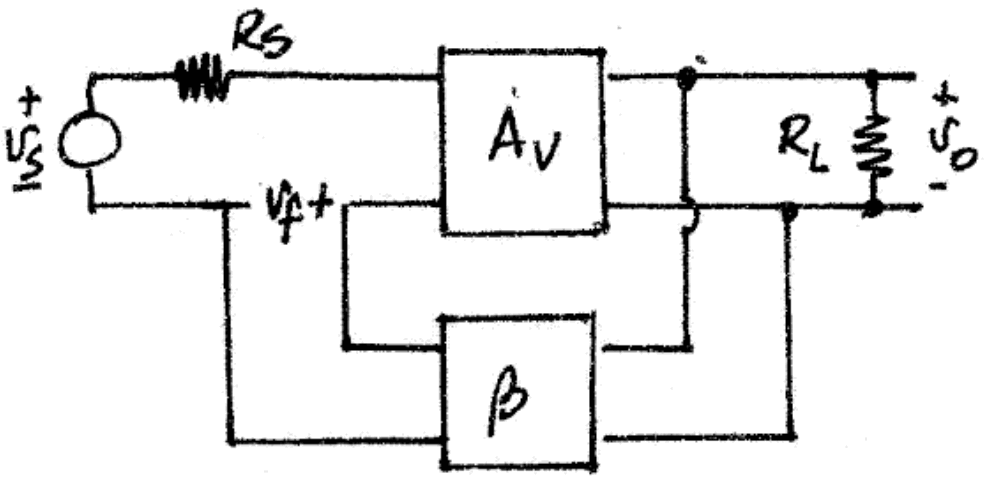
\includegraphics[width=0.8\linewidth]{_fig/retro_m-nodo_c-lazo.png}
	\caption{Muestreo de Nodo - Comparación de Lazo, Diagrama de Bloques}
	\label{fig:retro_m-nodo_c-lazo}
\end{figure}

En la Figura \ref{fig:retro_m-nodo_c-lazo}, se repite la Figura \ref{fig:retro_m-nodo_c-nodo} del diagrama de bloques general de este tipo de retroalimentación. En este caso el cuadripolo apropiado es el de los parámetros \( h \), que se muestra en la Figura \ref{fig:figura3.46}, ya que es el que tiene un nodo común a la salida y un lazo a la entrada.

\begin{figure}[h]
	\centering
	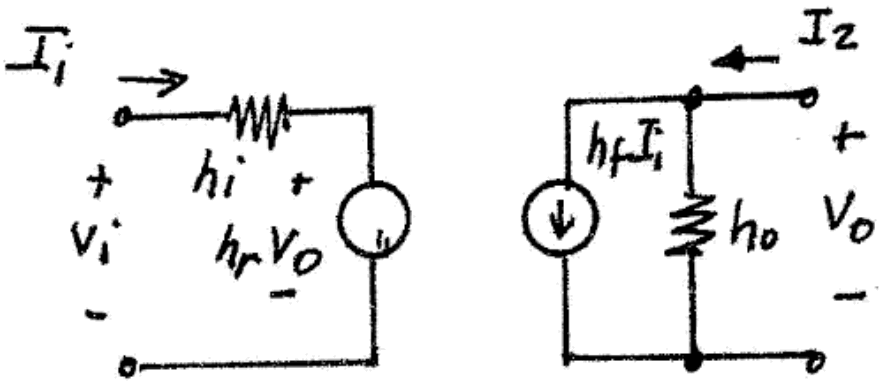
\includegraphics[width=0.8\linewidth]{_fig/retro_m-nodo_c-lazo_cuadripolo.png}
	\caption{Cuadripolo de parámetros \( h \).}
	\label{fig:retro_m-nodo_c-lazo_cuadripolo}
\end{figure}

Para el cuadripolo de los parámetros \( h \) se tiene:

\begin{equation}
	Vi = h_i I_i + h_r Vo \quad (3.23a)
\end{equation}

\begin{equation}
	I_2 = h_f I_i + h_o Vo \quad (3.23b)
\end{equation}

donde:

\( h_i = V_i / I_i \), con la salida en corto circuito.

\( h_r = V_i / V_o \), con la entrada abierta.

\( h_f = I_2 / I_i \), con la salida en corto circuito.

\( h_o = I_o / V_o \), con la entrada abierta.

Como en los casos anteriores, el manejo del análisis se simplifica tremendamente si se cumplen unas condiciones básicas:

\begin{equation}
	|h_i| \gg |h_f| \quad (3.24a)
\end{equation}

\begin{equation}
	|h_r| \gg |h_o| \quad (3.24b)
\end{equation}

\begin{equation}
	|h_i h_o| \gg |h_f h_r| \quad (3.24c)
\end{equation}

\begin{figure}[h]
	\centering
	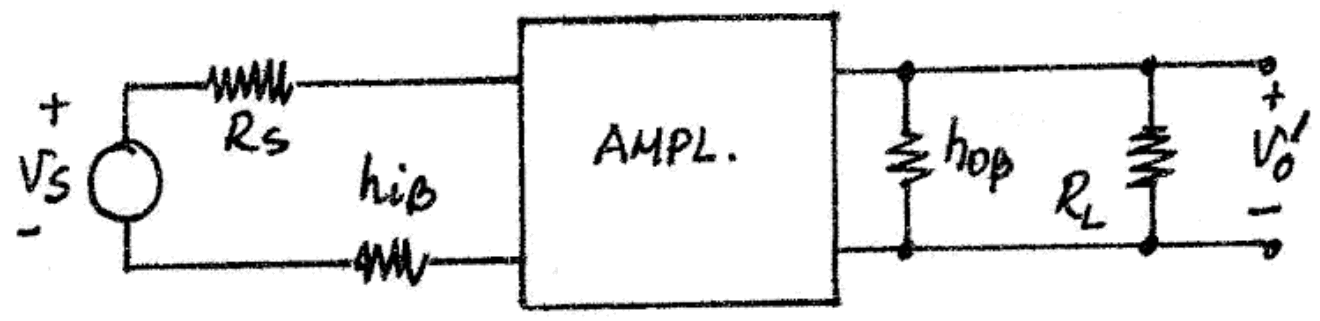
\includegraphics[width=0.8\linewidth]{_fig/retro_m-nodo_c-lazo_calcular-a.png}
	\caption{Circuito para calcular \( A \) sin retroalimentación.}
	\label{fig:retro_m-nodo_c-lazo_calcular-a}
\end{figure}

En la Figura \ref{fig:retro_m-nodo_c-lazo_calcular-a} se muestra cómo queda el circuito para calcular \( A \) sin retroalimentación, donde \( h_i \beta = V_i \beta / I_i \beta \) con \( V_o \beta = 0 \) y 
\( h_o \beta = 	I_{2\beta} / V_{o\beta} \) con \( V_{i\beta} = 0 \). Entonces: \( A_f = \frac{V_o}{V_s} = \frac{A}{1 + A \beta} \), donde \( A = -\frac{h_f A}{h_i h_o}, \quad \beta = -h_r \beta \)

\subsubsection{Ejemplo} %p163

Como ejemplo, se muestra otro amplificador con retroalimentación en la Figura \ref{fig:retro_m-nodo_c-lazo_ejm1a}.

\begin{figure}[h]
	\centering
	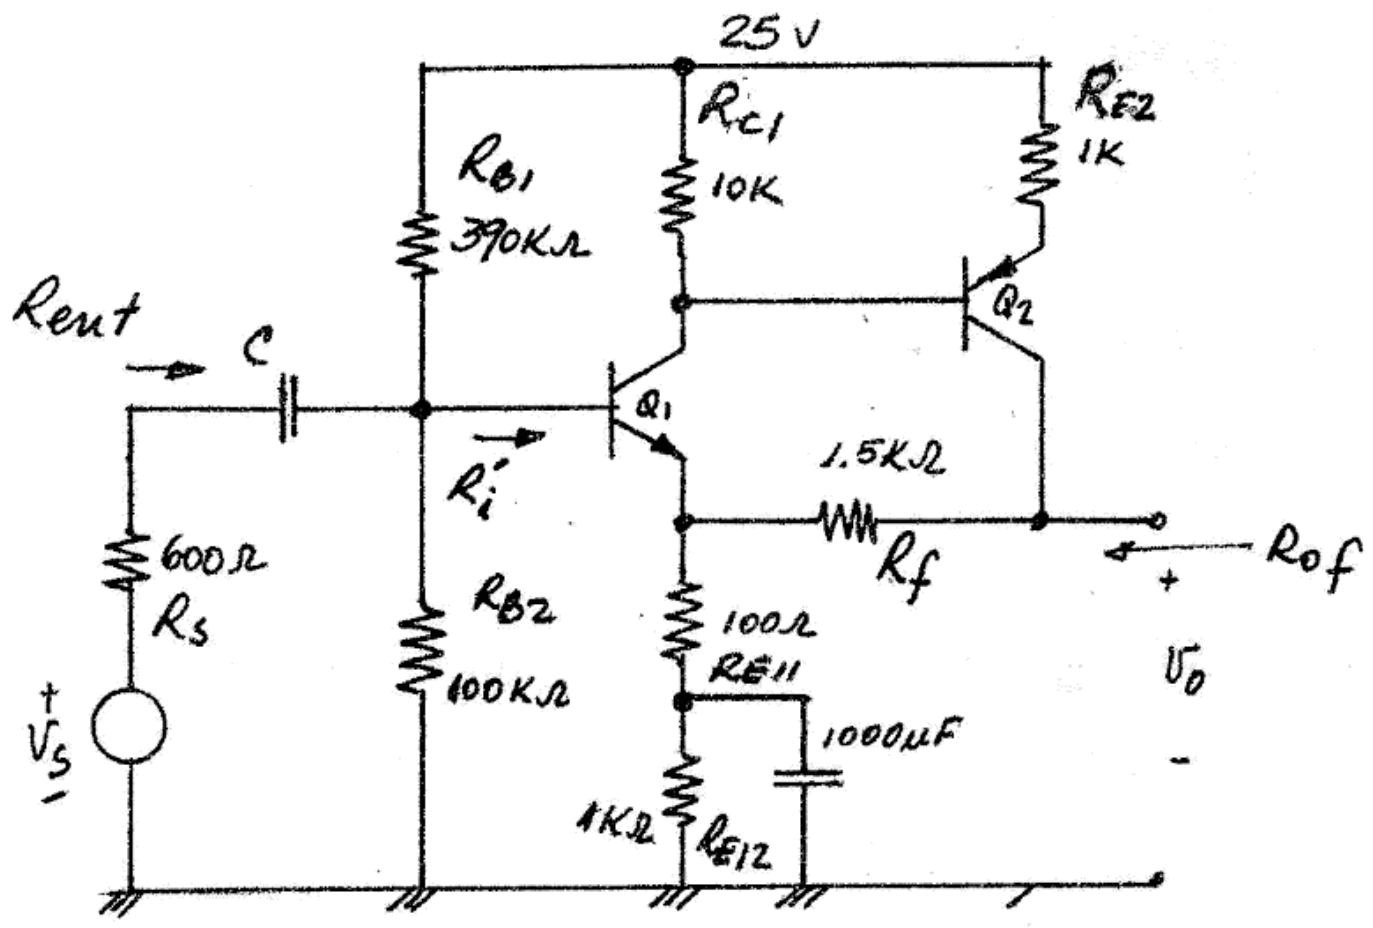
\includegraphics[width=0.8\linewidth]{_fig/retro_m-nodo_c-lazo_ejm1a.png}
	\caption{Ejemplo}
	\label{fig:retro_m-nodo_c-lazo_ejm1a}
\end{figure}

\textbf{Análisis según la Metodología de Retroalimentación}

\textbf{Primero:} \textit{Identificación del tipo de retroalimentación}:

La retroalimentación se crea por medio de la rama \( R_f \). Esta rama llega al lazo de entrada, y por lo tanto es \textbf{comparación de lazo}. En la salida, se toma la señal de retroalimentación en el mismo nodo de salida, por lo tanto es \textbf{muestreo de nodo}, es decir, se muestrea la tensión de salida.

\textbf{Segundo:} \textit{Hallar el punto de operación}:

En continua queda el circuito que se muestra en la Figura 3.49.

Una primera ecuación surge de la malla formada por la resistencia de colector de \( Q1 \) y la resistencia de emisor de \( Q2 \):

\[ (I_{C1} - I_{E2} \beta) \cdot 0k = I_{E2} \cdot 1k + 0.7 \]

Despejando \( I_{E2} \) queda:

\[ I_{E2} = \frac{V_{CC} - 0.7}{R_{E2} + R_{C1} (\beta + 1)} = 0.637 \text{ mA} \]

\begin{figure}[h]
	\centering
	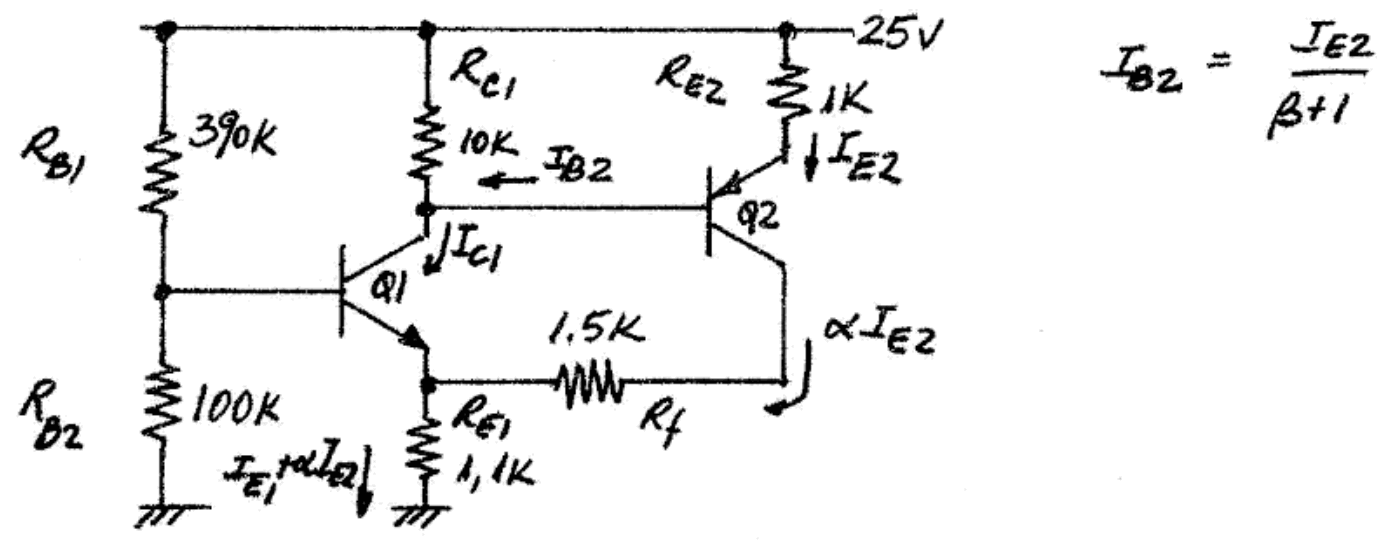
\includegraphics[width=0.8\linewidth]{_fig/retro_m-nodo_c-lazo_ejm1b.png}
	\caption{Circuito en DC de la Figura \ref{fig:retro_m-nodo_c-lazo_ejm1a}}
	\label{fig:retro_m-nodo_c-lazo_ejmb}
\end{figure}

Por otro lado, se convierte el circuito a la izquierda de la base de Q1 en su equivalente de Thevenin y se resuelve la malla resultante:

\[ 5.1 = \frac{80k I_{E1}}{\beta +1} + 0.7 + ( I_{E1} + \alpha I_{E2} 1.1k \]

Reemplazando la expresión de $I_{E2}$ de la ecuación anterior, se encuentra:

\[ I_{E1} = 435 \mu A \]

\[ I_{E2} = 3.28 mA \]

\begin{figure}[h]
	\centering
	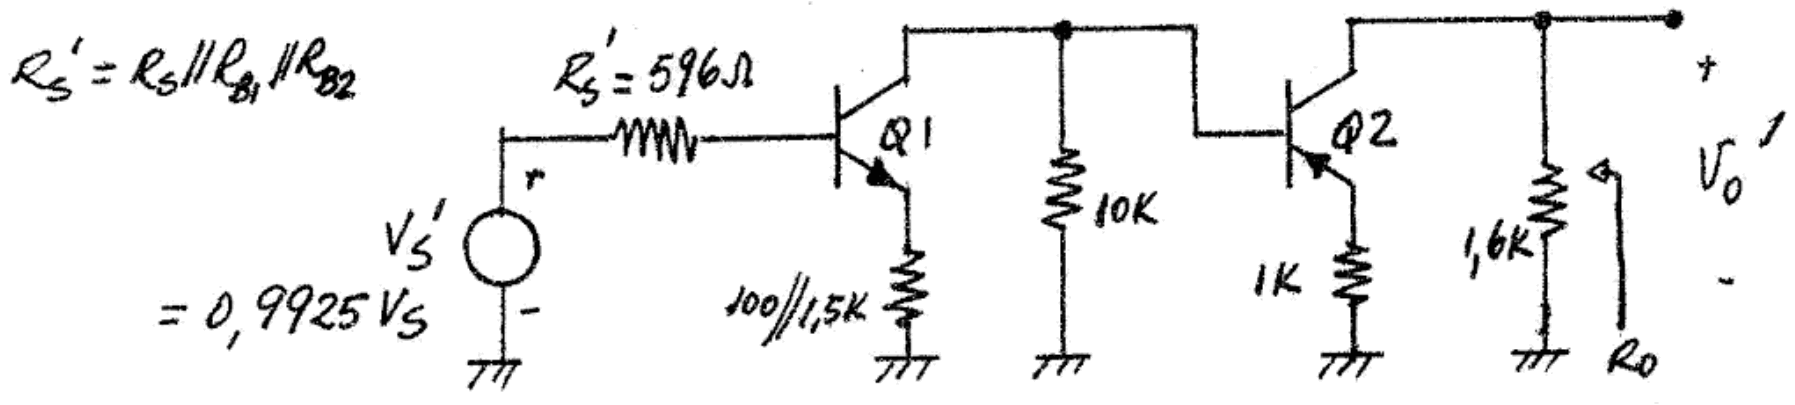
\includegraphics[width=0.8\linewidth]{_fig/retro_m-nodo_c-lazo_ejm1c.png}
	\caption{Circuito sin retroalimentación, parte A}
	\label{fig:retro_m-nodo_c-lazo_ejmc}
\end{figure}

\begin{figure}[h]
	\centering
	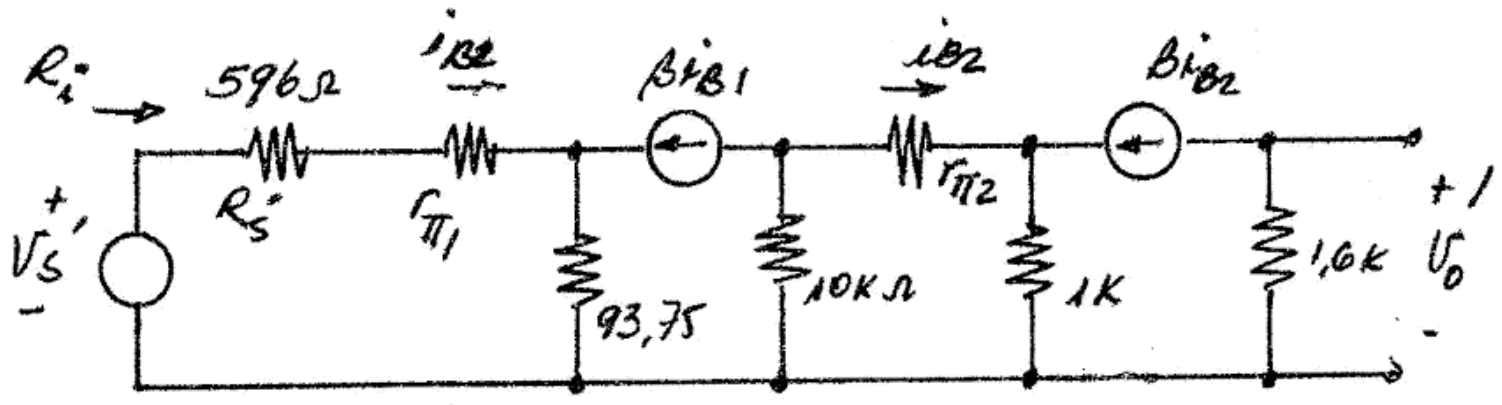
\includegraphics[width=0.8\linewidth]{_fig/retro_m-nodo_c-lazo_ejm1d.png}
	\caption{Circuito sin retroalimentación, parte B}
	\label{fig:retro_m-nodo_c-lazo_ejmd}
\end{figure}

\textbf{Tercero:} Con estos valores de los puntos de operación se pueden calcular los valores de los parámetros de los transistores. Se elimina la red de retroalimentación para dejar el amplificador sin retroalimentación, al cual se anexa a la entrada y a la salida el efecto de carga de la red de retroalimentación. El resultado se muestra en la Figura \ref{fig:retro_m-nodo_c-lazo_ejmc}, con su circuito equivalente a frecuencias medias en la Figura \ref{fig:retro_m-nodo_c-lazo_ejmd}.

Aqui se ha transformado \( R_{s} \) y las resistencias de polarización \( R_{B1} \) y \( R_{B2} \) junto con la fuente \( V_{s} \) en su equivalente de Thevenin con \( R_{s}^{\prime} \) y \( V_{s}^{\prime} \) para llegar a la configuración de la Fig. \ref{fig:retro_m-nodo_c-lazo_c}. De aqui procedemos normalmente para obtener:

\[A = \frac{v_{o}^{\prime}}{v_{s}^{\prime}} = 89.6\]

\[R_{i} = R_{s}^{\prime} + r_{\pi} + (\beta + 1) 93.75 = 16041 \Omega\]

\[R_{o} = 1.6 k\Omega\]

\begin{figure}[h]
	\centering
	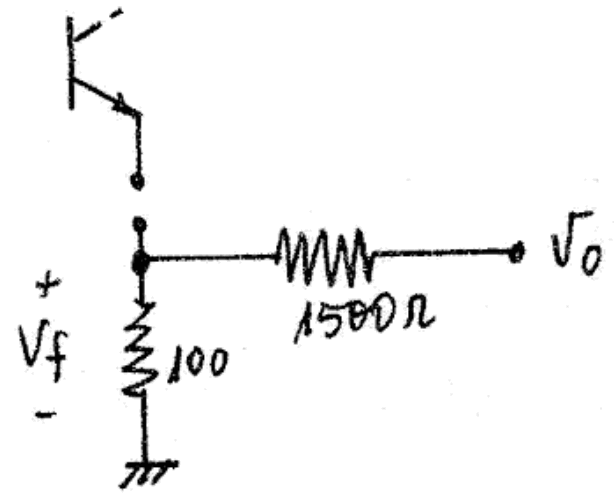
\includegraphics[width=0.5\linewidth]{_fig/retro_m-nodo_c-lazo_ejm1e.png}
	\caption{Circuito para determinar $\beta$}
	\label{fig:retro_m-nodo_c-lazo_ejme}
\end{figure}				
\textbf{Cuarto:}  La red de retroalimentación está formada por \( R_{EM} \) y \( R_{f} \), tal como se muestra en la Figura \ref{fig:retro_m-nodo_c-lazo_ejme}. \( \beta \) viene dada por \( \frac{v_{f}}{v_{o}} = \frac{R_{EM}}{R_{EM} + R_{f}} = \frac{100}{100 + 1500} = 0.0625 \)

\textbf{Quinto:}  Finalmente, una vez conocido todos los valores sin retroalimentación, se procede a calcular los valores con retroalimentación, y \( \beta \) se pueden determinar las características del circuito con retroalimentación. Tenemos:

\[ D = 1 + A\beta = 6.6 \]

\[ A_f = A/D = 13.6 \]

\[ R_{if} = R_i D = 106 k\Omega \]

\[ R_{of} = R_o / D = 242 \Omega \]

En la consideración final se encuentra el valor de la resistencia de entrada después de la fuente, $R_i^{\prime}$. Haciendo referencia a la ecuación desarrollada en la discusión de este tipo de retroalimentación, se obtiene:

\[ R_i^{\prime} = 105 k\Omega \quad R_{out} = 390k // 100k // 105k = 45.3 k\Omega \]

\subsection{Muestreo de Lazo - Comparación de Nodo} %p166

El último caso a considerar es la retroalimentación Muestreo de Lazo - Comparación de Nodo. En la Figura \ref{fig:retro_m-lazo_c-nodo}, se repite la Figura \ref{fig:retro_m-lazo_c-nodo_a} del diagrama de bloques general de este tipo de retroalimentación. En este caso el cuadripolo apropiado es el de los parámetros \( g \), que se muestra en la Figura \ref{fig:retro_retro_m-lazo_c-nodo_cuadripolo}, ya que es el que tiene un nodo común a la salida y un lazo a la entrada.

\begin{equation}
	I_1 = V_1 g_{11} + I_2 g_{12}
\end{equation}

\begin{figure}[h]
	\centering
	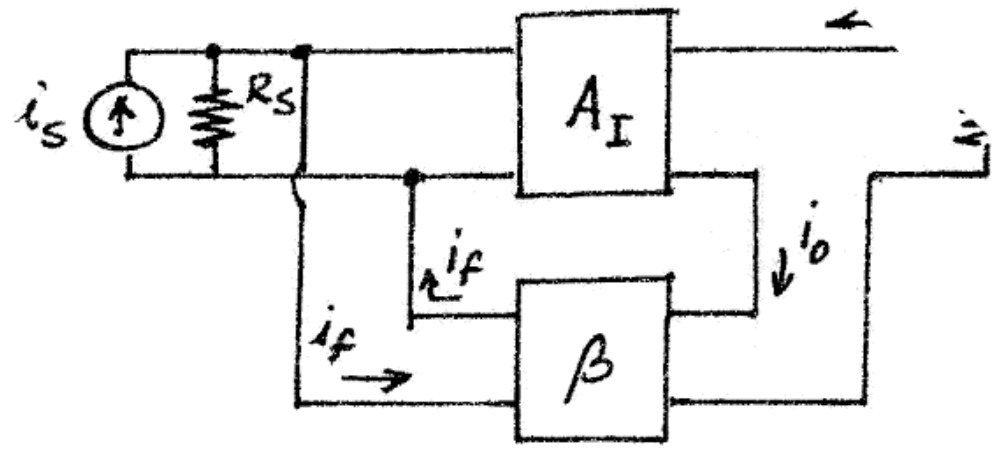
\includegraphics[width=0.8\linewidth]{_fig/retro_m-lazo_c-nodo.png}
	\caption{Muestreo de Lazo - Comparación de Nodo, Diagrama de Bloques}
	\label{fig:retro_m-lazo_c-nodo}
\end{figure}

\begin{figure}[h]
	\centering
	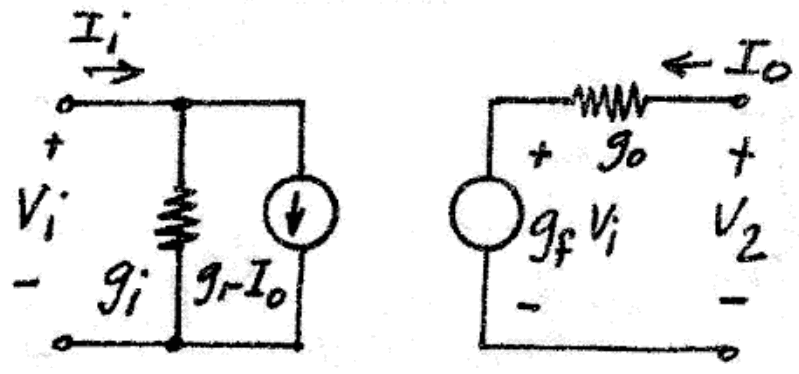
\includegraphics[width=0.6\linewidth]{_fig/retro_m-lazo_c-nodo_cuadripolo.png}
	\caption{Cuadripolo de parámetros \( g \).}
	\label{fig:retro_retro_m-lazo_c-nodo_cuadripolo}
\end{figure}

Para el cuadripolo de los parámetros \( g \) se tiene:

\begin{equation}
	V_2 = g_f V_i + g_o I_o
\end{equation}

Igual a los casos anteriores, el manejo del análisis se simplifica tremendamente si se cumplen unas condiciones básicas:

\begin{equation}
	|g_{fA}| >> |g_{f\beta}|
\end{equation}

\begin{equation}
	|g_{r\beta}| >> |g_{rA}|
\end{equation}

\begin{equation}
	|G_i G_o| >> |g_{fA} g_{rA}|
\end{equation}

\begin{figure}[h]
	\centering
	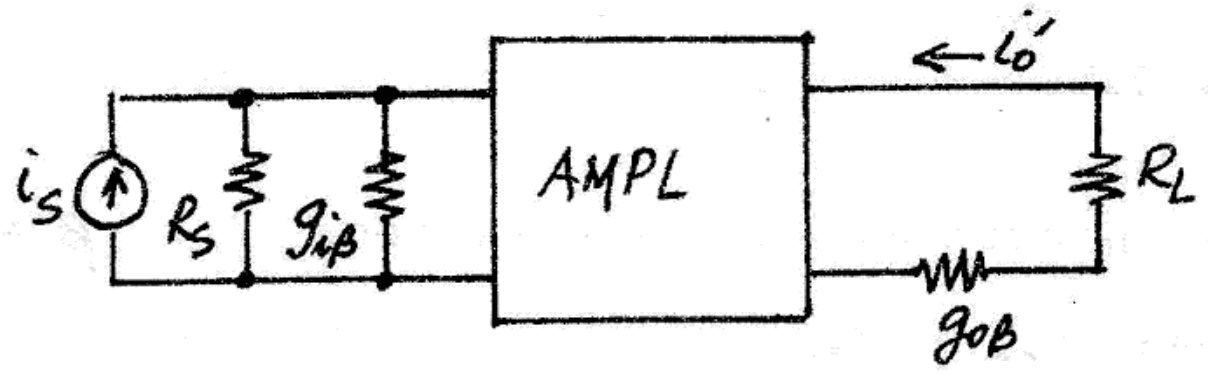
\includegraphics[width=0.6\linewidth]{_fig/retro_retro_m-lazo_c-nodo_calcular-a.png}
	\caption{Cuadripolo de parámetros \( g \).}
	\label{fig:retro_retro_m-lazo_c-nodo_calcular-a}
\end{figure}

En la Figura \ref{fig:retro_retro_m-lazo_c-nodo_calcular-a} se muestra cómo queda el circuito para calcular \( A \) sin retroalimentación. Entonces \( A_f = \frac{I_o}{V_s} = \frac{A}{(1 + A\beta)} \), donde \( A = \frac{-g_{fA}}{H_i H_o} \) y \( \beta = -g_r \beta \)

\subsubsection{Ejemplo} %p167

\begin{figure}[h]
	\centering
	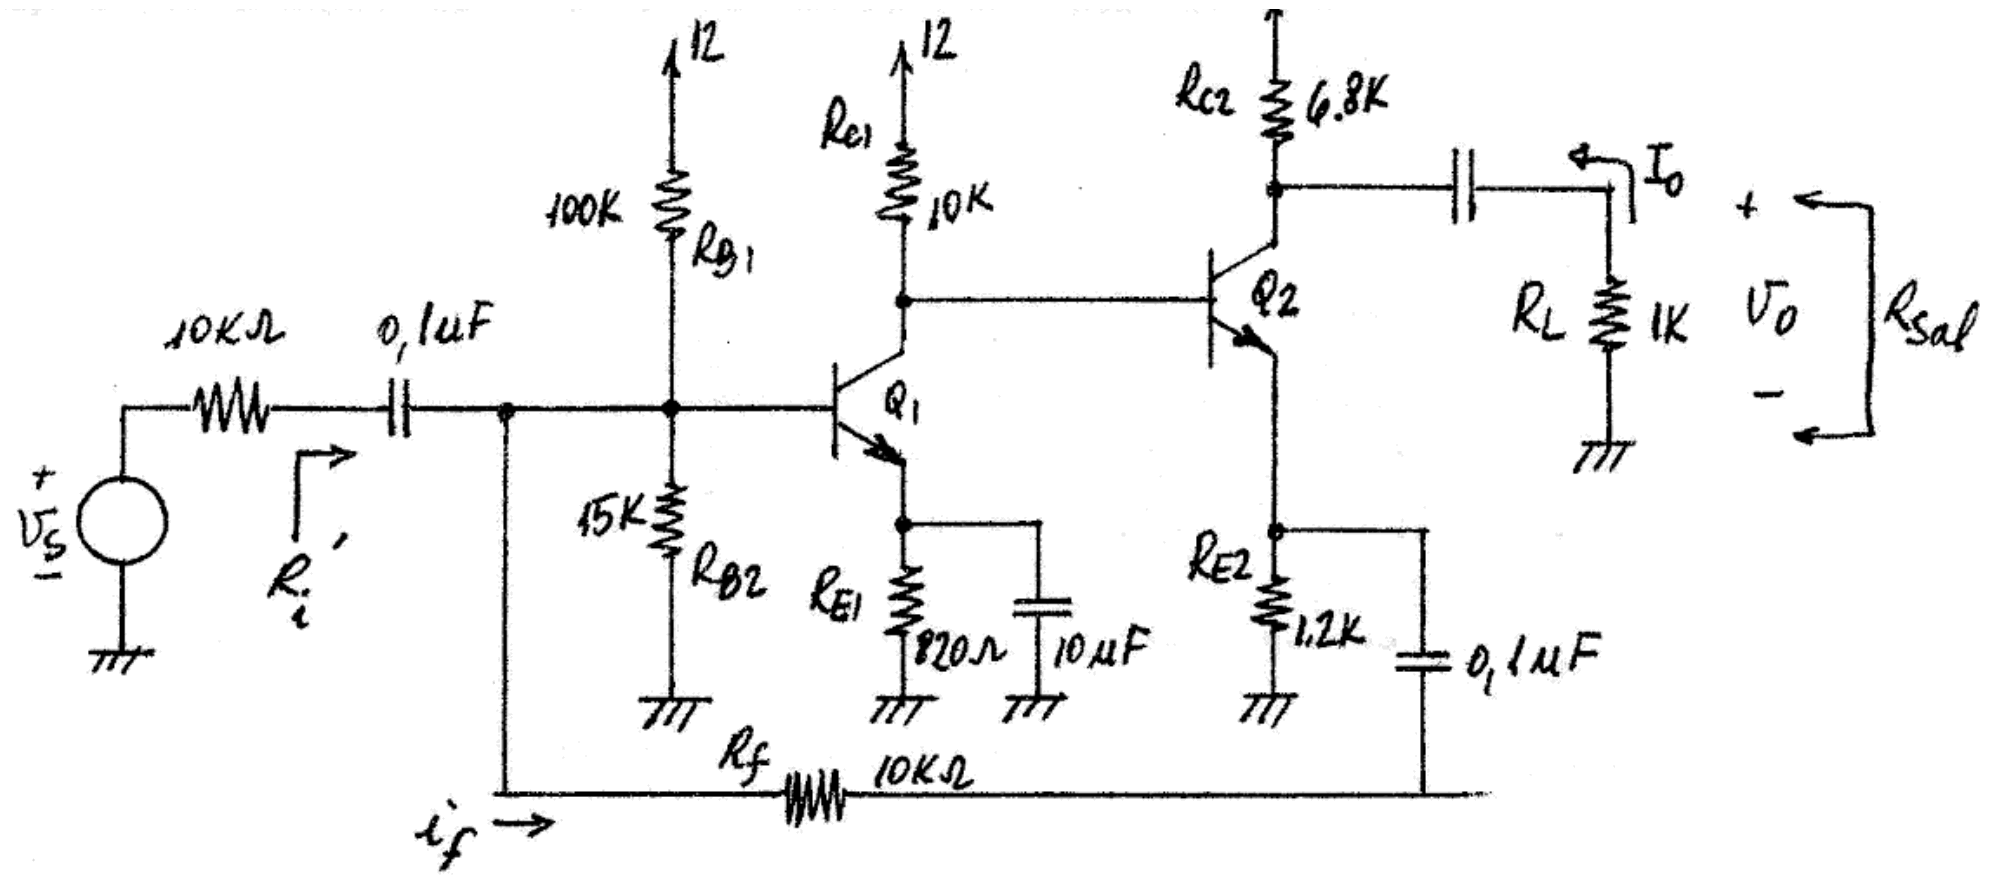
\includegraphics[width=0.8\linewidth]{_fig/retro_m-lazo_c-nodo_ejm1a.png}
	\caption{Circuito de ejemplo}
	\label{fig:retro_m-lazo_c-nodo_ejm1a}
\end{figure}

Ahora resolveremos un ejemplo con este tipo de retroalimentación, que se muestra en la Figura \ref{fig:retro_m-lazo_c-nodo_ejm1a}.

\textbf{Primero:} identificar el tipo de retroalimentación: la retroalimentación se crea por medio de la rama Rf. Esta rama llega al mismo nodo de entrada, y por lo tanto es comparación de nodo. En la salida, la tensión en Re2 nos da una muestra del valor de la corriente en el lazo de salida, y por lo tanto es muestreo de lazo.

\textbf{Segundo:} Hallar el punto de operación. En continua queda el circuito que se muestra en la Figura \ref{fig:retro_m-lazo_c-nodo_ejm1a}.

\begin{figure}[h]
	\centering
	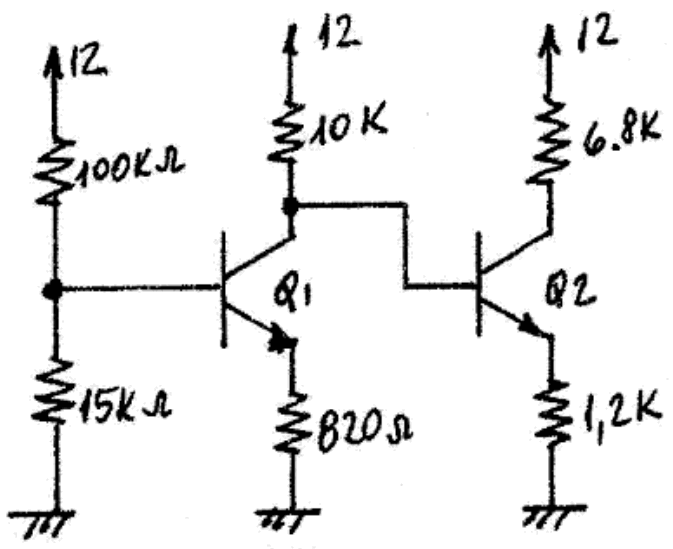
\includegraphics[width=0.5\linewidth]{_fig/retro_m-lazo_c-nodo_ejm1b.png}
	\caption{Circuito en DC de la Figura \ref{fig:retro_m-lazo_c-nodo_ejm1a}}
	\label{fig:retro_m-lazo_c-nodo_ejm1b}
\end{figure}

Aplicando el procedimiento de costumbre, con \( \beta = 130 \), \(r_T = 3.4k\Omega \), se obtiene:

\[
(V_{CE1}, I_{C1}) \approx (1.2V, 1mA)
\]

\[
(V_{CE2}, I_{C2}) \approx (3.5V, 1.06mA)
\]

\textbf{Tercero:} Con estos valores de los puntos de operación se pueden calcular los valores de los parámetros de los transistores. Se elimina la red de retroalimentación para dejar el amplificador sin retroalimentación, al cual se anexa a la entrada y a la salida el efecto de carga de la red de retroalimentación. El resultado se muestra en la Figura \ref{fig:retro_m-lazo_c-nodo_ejm1c}, con su circuito equivalente a frecuencias medias en la Figura \ref{fig:retro_m-lazo_c-nodo_ejm1d}.

\begin{figure}[h]
	\centering
	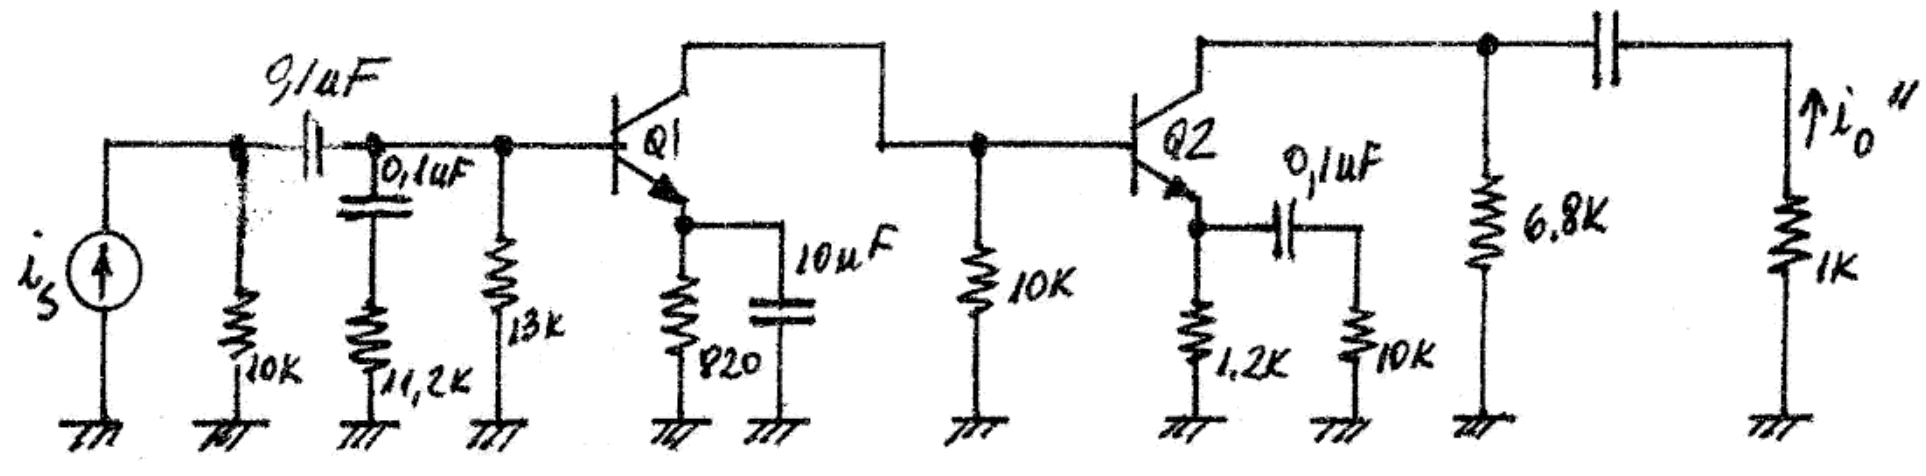
\includegraphics[width=0.8\linewidth]{_fig/retro_m-lazo_c-nodo_ejm1c.png}
	\caption{Circuito sin retroalimentación. Parte 1}
	\label{fig:retro_m-lazo_c-nodo_ejm1c}
\end{figure}

\begin{figure}[h]
	\centering
	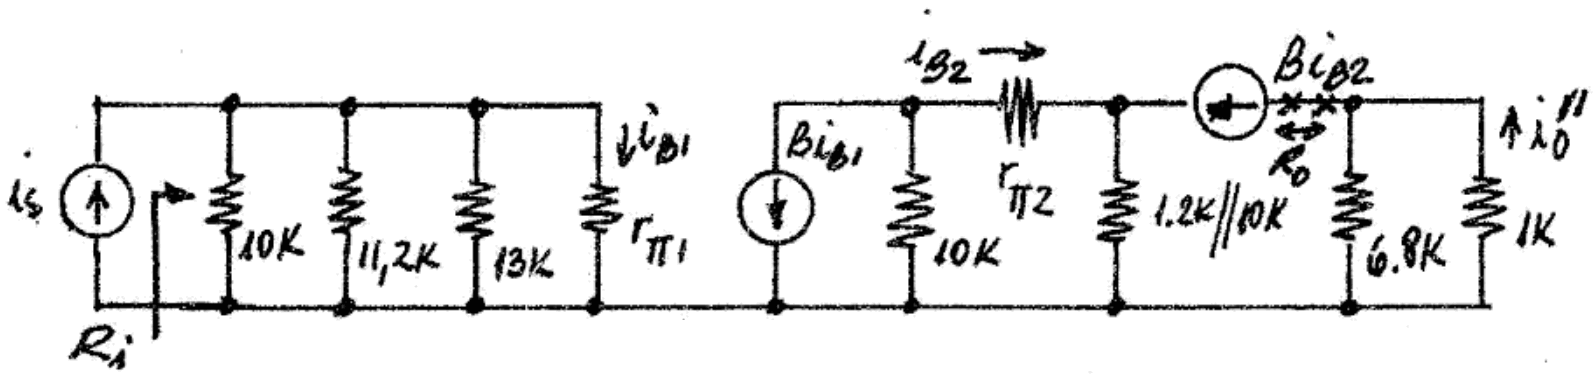
\includegraphics[width=0.8\linewidth]{_fig/retro_m-lazo_c-nodo_ejm1d.png}
	\caption{Circuito sin retroalimentación. Parte 2}
	\label{fig:retro_m-lazo_c-nodo_ejm1d}
\end{figure}

Se hace notar que hemos convertido la fuente de entrada, junto con su resistencia, en el equivalente de Norton por considerarse de una retroalimentación tipo comparación de nodo. De aquí procedemos normalmente para obtener:

\[ A = \frac{i_o^{''}}{i_s} = -503 \]

\[ R_i\prime = 1785 \]

\[ R_o = \infty \]

De querer la respuesta de frecuencia sin retroalimentación, se volverían a colocar los condensadores para frecuencias bajas, y para altas se trabajaría con el modelo de alta del transistor.

\textbf{Cuarto:} La red de retroalimentación está formada por $R_f$ y $R_{E2}$. El factor de retroalimentación $\beta$ viene dado por $\frac{i_f}{i_o}$. Sin embargo, se hace notar que la corriente que circula por $R_{E2}$ no es exactamente la corriente de salida $i_o$, por dos motivos: la corriente de emisor es ligeramente mayor que la corriente de colector, y además, la corriente de colector es la suma de la corriente de salida más la corriente que circula por la resistencia de colector. En la Figura \ref{fig:retro_m-lazo_c-nodo_ejm1e_a} se muestra propiamente la red de retroalimentación; de aquí se obtiene \( \frac{i_f}{i_o}\prime = \frac{R_{E2}}{R_{E2}+R_f} \). En la figura \ref{fig:retro_m-lazo_c-nodo_ejm1e_b} se muestra la etapa de salida para determinar la relación entre la corriente de salida $i_o$ y l acorriente de emisor. Entonces la relación entre la corriente de salida y la corriente de retroalimentación, es decir, $\beta$ viene dada por:

\[ \frac{i_f}{i_o} = (-0.107)(1.15) = -0.123	\]

\begin{figure}[h]
	\centering
	\subfloat[A]
	{
		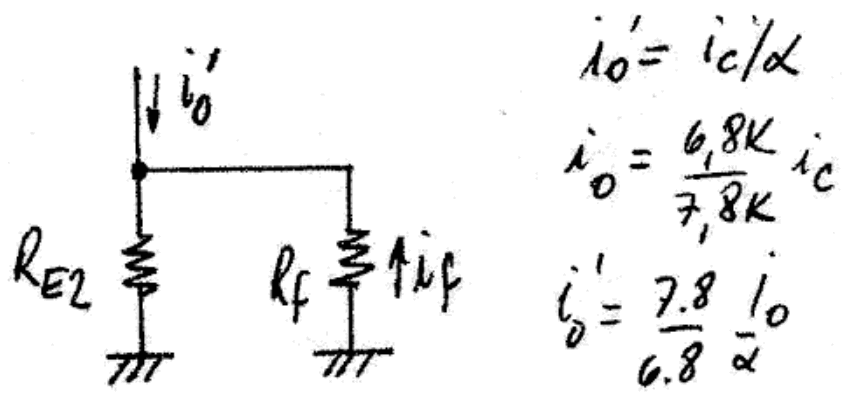
\includegraphics[width=0.5\linewidth]{_fig/retro_m-lazo_c-nodo_ejm1e_a.png}
		\label{fig:retro_m-lazo_c-nodo_ejm1e_a}
	}
	\subfloat[B]
	{
		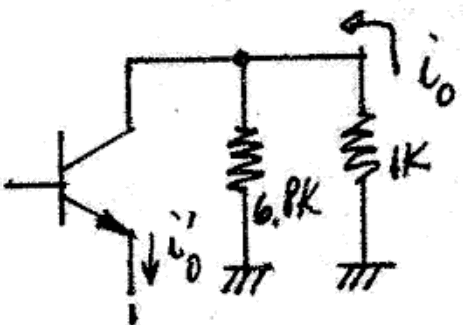
\includegraphics[width=0.3\linewidth]{_fig/retro_m-lazo_c-nodo_ejm1e_b.png}
		\label{fig:retro_m-lazo_c-nodo_ejm1e_b}
	}
	\caption{Circuitos para determinar $\beta$}
	\label{fig:retro_m-lazo_c-nodo_ejm1e}
\end{figure}

\textbf{Quito:} Finalmente, una vez conocidos todos los valores sin retroalimentación y \( \beta \), se pueden determinar las características del circuito con retroalimentación. Tenemos:

\[ D = 1 + A\beta = 62.7 \]

\[ A_f = \frac{A}{D} = -8 \]

\[ R_{if} = \frac{R_i}{D} = 28.4 \]

\[ R_{of} = R_o D = \infty \]

\[ \frac{v_o}{v_s} = -\frac{i_o R_L}{i_s R_s} = \frac{-A_f R_L}{R_s} = 0.8 \]

En los ajustes finales se encuentran valores de las características de mayor interés, como son la resistencia de entrada después de la fuente, \( R_i' \) y la resistencia de salida total, $R_{sal}'$. Haciendo referencia a las ecuaciones desarrolladas en la discusión de este tipo de retroalimentación, se obtiene:

\[ R_i\prime = \frac{1}{\frac{1}{28.4} - \frac{1}{10k}} = 28.5 \Omega \]

\[ R_{sal} = 1k \parallel 6.8k = 872 \Omega \]

\subsection{Resumen} %p171

Si se satisfacen las condiciones de que la amplificación es principalmente por el amplificador, y que la retroalimentación es principalmente por la red de retroalimentación, como por ejemplo en las ecuaciones \ref{equ:retro_m-nodo_c-nodo_admitancia-yfA}, \ref{equ:retro_m-nodo_c-nodo_admitancia-yfB} y 			\ref{equ:retro_m-nodo_c-nodo_admitancias}, entonces puede utilizarse la Metodología de Retroalimentación que consta de los siguientes pasos:

\begin{enumerate}
	\item Identificación del tipo de retroalimentación.
	\item Generalmente se tiene que encontrar el punto de operación, para el cual se trabaja con el circuito original, sin modificaciones.
	\item Formación del amplificador sin retroalimentación, del cual se determina la ganancia sin retroalimentación, \( A \), la resistencia de entrada sin retroalimentación, \( R_{if} \), la resistencia de salida sin retroalimentación, \( R_{of} \), y las frecuencias de corte baja y corte alta sin retroalimentación, \( f_L \) y \( f_H \) respectivamente.
	\item El cálculo de \( \beta \) de acuerdo a los lineamientos que se han dado.
	\item El cálculo de las características del circuito con retroalimentación de acuerdo a las siguientes relaciones:
\end{enumerate}

\begin{equation}
	A_f = \frac{A}{1 + A\beta}
\end{equation}

\begin{equation}
	R_{if} =
	\begin{cases} 
		R_i/(1 + A\beta) & \text{si es comparación de nodo} \\
		R_i(1 + A\beta) & \text{si es comparación de lazo}
	\end{cases}
\end{equation}

\begin{equation}
	R_{of} =
	\begin{cases} 
		R_o/(1 + A\beta) & \text{si es muestreo de nodo} \\
		R_o(1 + A\beta) & \text{si es muestreo de lazo}
	\end{cases}
\end{equation}

\begin{equation}
	f_{Lf} = \frac{f_L}{1 + A\beta}
\end{equation}

\begin{equation}
	f_{Hf} = f_H (1 + A\beta)
\end{equation}

\section{Determinación de configuraciones de retroalimentación positiva} %p171

En ocasiones se presentan configuraciones que tienen retroalimentación, pero de tal forma que en lugar de restar el nivel de la señal de entrada, más bien lo aumentan. Esto corresponde a una situación inestable, se entra en un círculo vicioso ya que la misma señal realimentada aumenta la entrada, que aumenta la señal de salida y así sucesivamente.

Una forma de determinar si una configuración tiene retroalimentación positiva o negativa consiste en encontrar valores de \( A \) y \( \beta \) siguiendo los procedimientos que hemos formulado, y comparar los signos de \(A\) y \(\beta\):

\begin{itemize}
	\item Si son iguales, tenemos retroalimentación negativa.
	\item Si son opuestos, tenemos retroalimentación positiva.
\end{itemize}

Sin embargo, para comprobaciones rápidas se propone otra manera, que a su vez, nos da una concepción más intuitiva de por qué la retroalimentación negativa le imparte una estabilidad a un sistema.

El método consiste en abrir el lazo de retroalimentación en cualquier punto y aplicar una fuente imaginaria a ese punto; se hace un seguimiento de esta señal alrededor del lazo, y si al regresar al punto de partida, es decir, el punto donde se abrió el lazo, la señal está en contrafase, tenemos un caso de retroalimentación negativa. Si, en cambio, la señal que retorna está en fase con la señal aplicada, entonces tenemos retroalimentación positiva.

Este método se demuestra aplicado a los circuitos de la Figura \ref{fig:retro_pos_ejm1}.

\begin{figure}[h]
	\centering
	\subfloat[Paso 1]
	{
		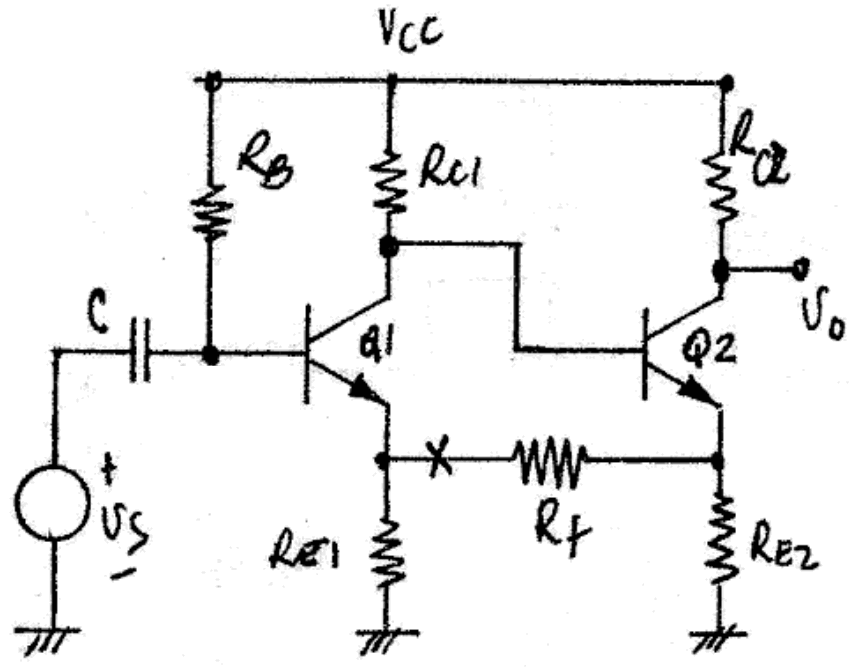
\includegraphics[width=0.22\linewidth]{_fig/retro_pos_ejm1a.png}
		\label{fig:retro_pos_ejm1a}
	}
	\subfloat[Paso 2]
	{
		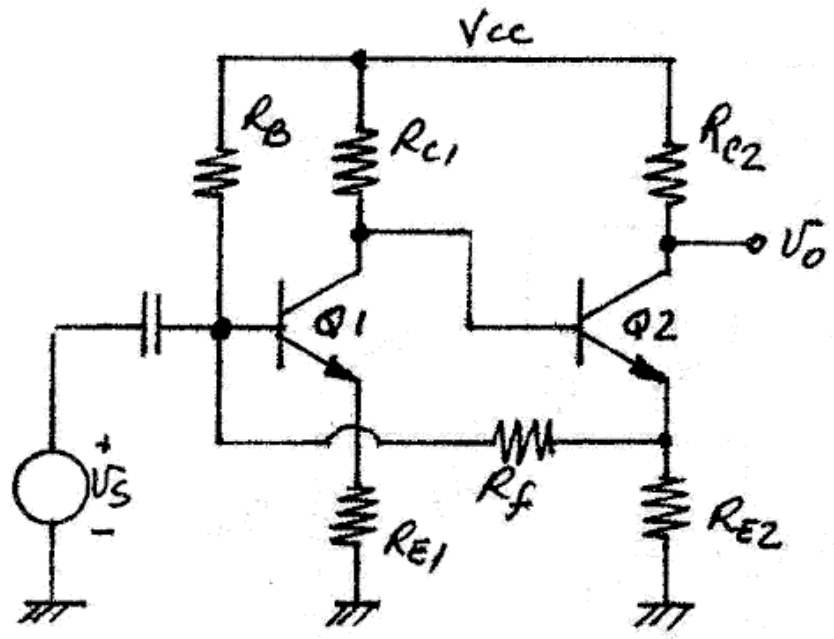
\includegraphics[width=0.22\linewidth]{_fig/retro_pos_ejm1b.png}
		\label{fig:retro_pos_ejm1b}
	}
	\subfloat[Paso 3]
	{
		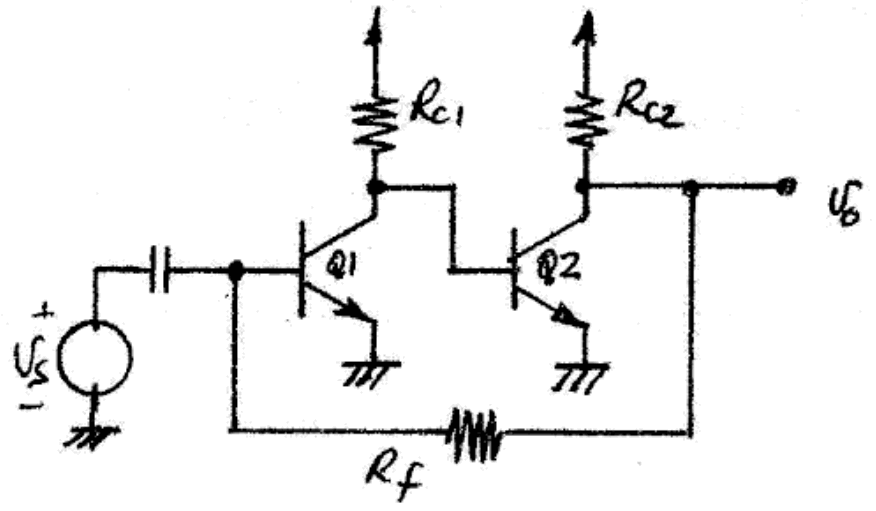
\includegraphics[width=0.22\linewidth]{_fig/retro_pos_ejm1c.png}
		\label{fig:retro_pos_ejm1c}
	}
	\subfloat[Paso 4]
	{
		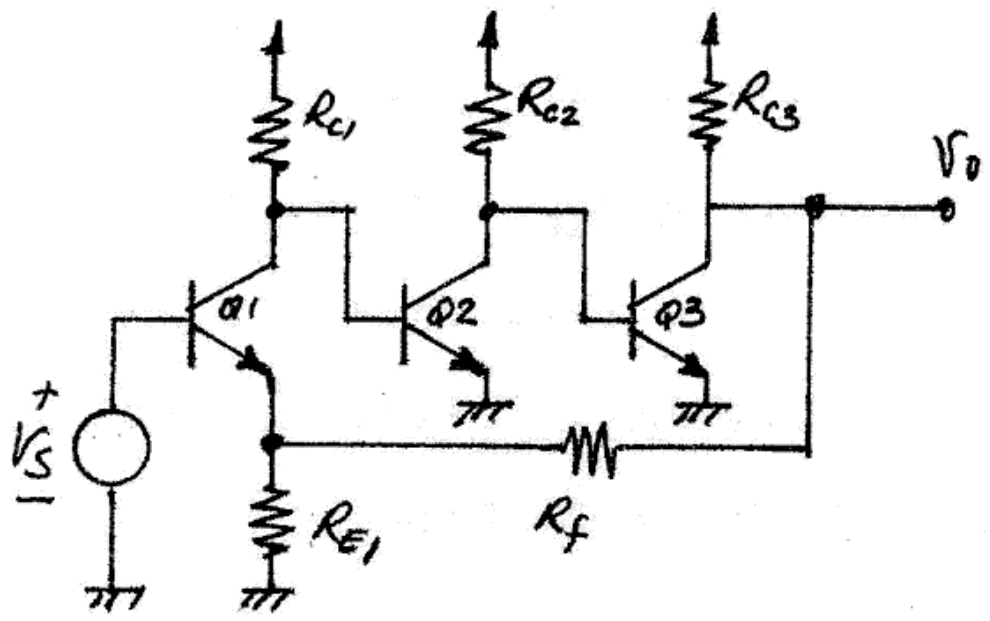
\includegraphics[width=0.22\linewidth]{_fig/retro_pos_ejm1d.png}
		\label{fig:retro_pos_ejm1d}
	}
	\caption{Ejemplo 1: circuito con transistores}
	\label{fig:retro_pos_ejm1}
\end{figure}

En el circuito de la figura \ref{fig:retro_pos_ejm1a}, abrimos el lazo en el punto marcado con $x$. Se aplica una fuente de tensión al emisor de $Q_1$; el circuito queda como se muestra en la figura \ref{fig:retro_pos_ejm1a}. De esta forma, $Q_1$ queda como una base común, en donde de emisor a colector no hay inversión de fase. Luego, desde el colector de $Q_1$ (base de $Q_2$ al emisor de $Q_2$ tampoco hay inversión de fase. Finalmente, a través de la resistencia $R_f$ tampoco hay inversión de fase. Concluimos que la señal está en fase con la señal aplicada, indicando retroalimentación positiva.

Analice los demás circuitos de la figura \ref{fig:retro_pos_ejm1} y determine si son de retroalimentación positiva o negativa.

Finalmente, si se carga apropiadamente el lazo con la resistencia que vería la señal al seguir dando la vuelta al lazo, y se encuentra la relación entre la señal retornada a la señal aplicada, \( \frac{V_r}{V_a} \); se ha encontrado la \textbf{ganancia del lazo}, $A\beta$. La ganancia de lazo es muy utilizada para determinar la estabilidad de un sistema. Esto se realiza al circuito de la figura \ref{fig:retro_pos_ejm2a} para llegar a la figura \ref{fig:retro_pos_ejm2b}.

\begin{figure}[h]
	\centering
	\subfloat[Circuito con retroalimentación]
	{
		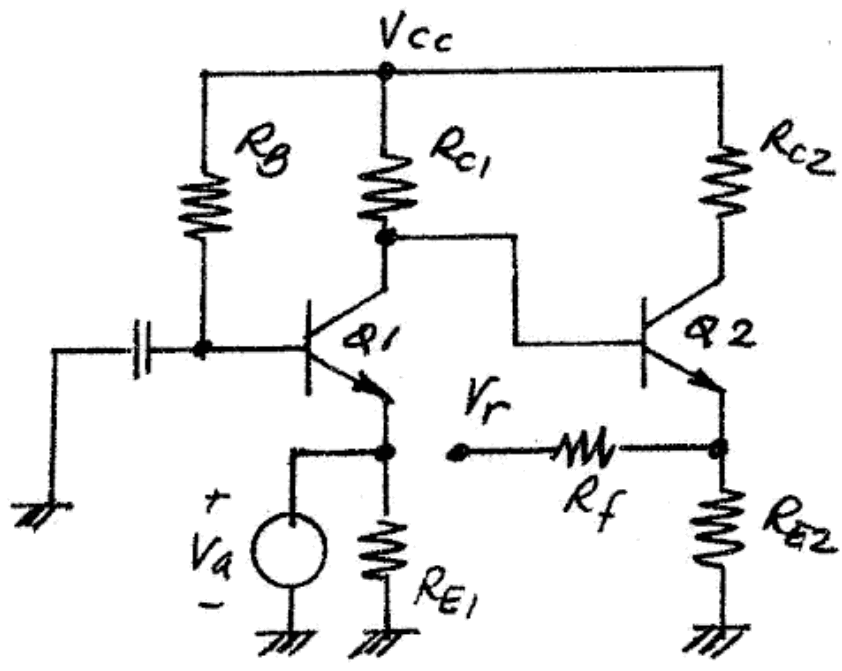
\includegraphics[width=0.4\linewidth]{_fig/retro_pos_ejm2a.png}
		\label{fig:retro_pos_ejm2a}
	}
	\subfloat[Análisis de retroalimentación]
	{
		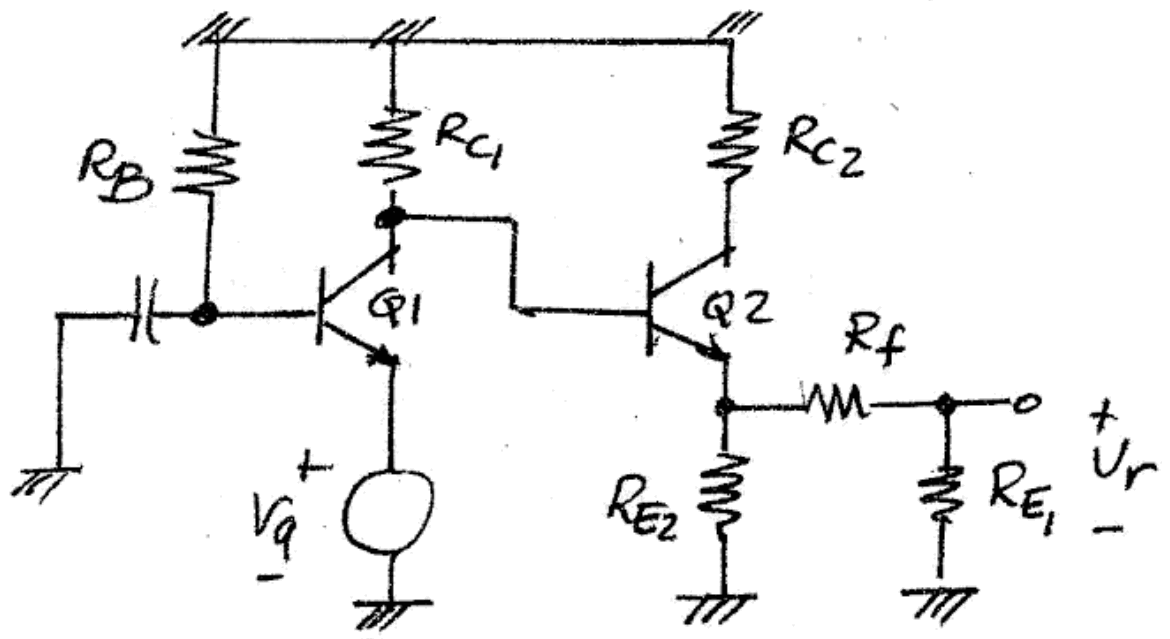
\includegraphics[width=0.5\linewidth]{_fig/retro_pos_ejm2b.png}
		\label{fig:retro_pos_ejm2b}
	}
	\caption{Ejemplo 2: circuito y analisis}
	\label{fig:retro_pos_ejm2}
\end{figure}

\textbf{Bibliografía:}

\begin{itemize}
	\item Millman, Halkias, \textit{Electrónica Integrada}, McGraw-Hill, 1972, Capítulo 13.
	\item Gray, Searle, \textit{Principios de Electrónica}, Wiley and Sons, 1969, Capítulo 18.
	\item Sedra, Smith, \textit{Microelectronic Circuits}, Holt-Saunders International Edition, New York, 1982, Capítulo 12.
\end{itemize}

\section{Problemario} %p175
- pendiente en apuntes -